\chapter{Resultados y Discusión de Resultados}
%\textbf{Should include a reiteration of the experiments, and their outcome.  Together with a description (discussion).  Preamble should include a reminder of the aims and objectives together with a list of experiments to achieve these.  Should include many charts and other visualization with appropriate descriptions}.  

\section{Extracciones líquido-sólido}\label{sec:Resultsliqsol}\index{Extracción!líquido-sólido}\index{Extractantes}
Inicialmente se prepararon membranas de 100~mg, de composición 33.3\% polímero base (CTA), 33.3\% plastificante (NPOE) y 33.4\% de cada una de las seis combinaciones posibles de los extractantes ácidos (LIX-54-100 y D2EHPA) con los extractantes neutros (T2EHP, Cyanex~923 y TBP), mezclados en proporción másica 1:1. Adicionalmente se preparó una membrana de 80~mg sin extractantes (60\% polímero base y 40\% plastificante) con fines comparativos. Se usaron 25~g de una fase donadora que contenía iones litio a una concentración de 40~mg~kg\mnn\ ($\sim$1.44\e{-4}~mol~kg\mnn) en hidróxido de sodio 0.04~mol~kg\mnn. La fase receptora fue de 30~g de ácido clorhídrico 0.4~mol~kg\mnn.

Los extractantes de las membranas preparadas y la concentración de litio en la fase receptora al final del proceso extractivo\footnote{La concentración inicial en esta fase es cero.} se muestran en la Tabla \ref{tab:liqsol1}. No se observó una disminución estadísticamente significativa en la concentración de litio en la fase donadora como consecuencia de la extracción. 

\begin{center}\begin{minipage}{0.65\textwidth}\begin{table}[H]
        \centering\footnotesize
        \begin{tabular}{@{}lllc@{}}\toprule
            \multirow{2}{*}{\textbf{ID}}&\multicolumn{2}{c}{\textbf{Extractantes}}&\textbf{Conc. \ce{Li^+}}\\
            &\textbf{Ácido} & \textbf{Quelante} & (mg~kg\mnn)\\\midrule
            \textbf{A.1}&\textbf{LIX-54-100}     & \textbf{TEHP}       &  \textbf{0.18}\\
            \textbf{A.2}&               & C\textbf{yanex 923} &  \textbf{0.33}\\
            A.3&               & TBP        &  0.03\\
            A.4&D2EHPA         & TEHP       &  0.05\\
            A.5&               & Cyanex~923 &  0.06\\
            A.6&               & TBP        &  >0.03\\
            A.7&\multicolumn{2}{l}{\textit{(Sin extractantes)}}&>0.03\\\bottomrule
        \end{tabular}
        \caption[Resultados extracción líquido-sólido (etapa I).]{Concentración final de litio en la fase receptora con la extracción líquido-sólido (etapa I).}
        \label{tab:liqsol1}
\end{table}\end{minipage}\end{center}

Las membranas probadas no extraen eficientemente el litio de la disolución donadora bajo las condiciones del experimento. En el mejor de los casos (membrana A.2), la eficiencia del sistema considerando la cantidad de litio que llega a la fase receptora respecto a la que hay inicialmente en la fase donadora es de 1.2\%. Considerando que en las membranas utilizadas hay cerca de 5\e{-5}~mol de cada extractante y que la fase donadora contiene 1.4\e{-4}~mol  del litio, asu\-miendo una estequimetría 1:1 del complejo formado por ambos extractantes con el litio, la eficiencia máxima posible para la extracción es de aproximadamente 35\%. La eficacia\footnote{Eficiencia relativa a la cantidad de extractante presente en la membrana.} de las membranas A.1 y A.2 es de 2.2 y 3.3\%, respectivamente. 

En una segunda fase, se prepararon membranas de 86~mg con las mezclas de extractantes que mostraron mejor desempeño en la fase inicial (LIX-54-100/Cyanex~923 y LIX-54-100/TEHP). Estos extractantes fueron probados en combinación e individualmente para comprobar la presencia de efectos sinérgicos cuando se usan en combinación. La proporción de los componentes de la membrana fue cambiada a 46\%, 35\% y 19\% para el polímero base, el plastificante y los extractantes, respectivamente. La fase donadora empleada (25~g) contenía iones litio a una concentración de 18~mg~kg$^{-1}$ en hidróxido de sodio 0.017~mol~kg$^{-1}$. La fase receptora fue de 15~g de ácido clorhídrico 0.1~mol~kg$^{-1}$. Los resultados obtenidos se muestran en la Tabla \ref{tab:liqsol2}.

\begin{center}\begin{minipage}{0.65\textwidth}\begin{table}[H]
        \centering\footnotesize
        \begin{tabular}{@{}llc@{}}\toprule
            \multirow{2}{*}{\textbf{ID}}&\multirow{2}{*}{\textbf{Extractantes}}&\textbf{Conc. \ce{Li^+}}\\
             && (mg~kg\mnn)\\\midrule
            B.1&LIX-54-100/TEHP       & 0.06\\
            \textbf{B.2}&\textbf{LIX-54-100/Cyanex~923}& \textbf{1.36}\\
            B.3&LIX-54-100            &  >0.03\\
            B.4&TEHP                  &  >0.03\\
            B.5&Cyanex~923            &  >0.03\\\bottomrule
        \end{tabular}
        \caption[Resultados extracción líquido-sólido (etapa II).]{Concentración final de litio en la fase receptora con la extracción líquido-sólido (etapa II).}
        \label{tab:liqsol2}
\end{table}\end{minipage}\end{center}

Las membranas con sólo un extractante en su composición son incapaces de extraer litio de una manera medible bajo las condiciones del experimento realizado. La PIM con la mezcla LIX-54-100/Cyanex~923 presenta un desempeño muy superior a la PIM con la mezcla LIX-54-100/TEHP (eficacias de 0.3 y 6.0 para las membranas B.1 y B.2, respectivamente). 

La mezcla de extractantes LIX-54-100/Cyanex~923 fue reportada por \citet{Pranolo2015} para la extracción de litio a partir de salmueras alcalinas por medio de \ac{SSX} usando ShellSol D70 (compuesto principalmente de alcanos lineales C11-C14 y alcanos cíclicos \citep{Shell2016}) como disolvente. Los autores determinaron que la estequiometría del aducto formado es 1:1 res\-pecto a ambos extractantes, pero reportan que la relación molar óptima LIX-54-100/Cyanex~923 es 2:1. El recobro de litio se logró de manera eficiente y con buena selectividad frente al sodio usando ácido clorhídrico 0.17~mol~L\mnn\ como disolución de recuperación. Esto sugiere que una pequeña concentración de ácido es suficiente para liberar el litio del complejo formado con los extractantes.

Con base en los resultados obtenidos, se decide que la optimización del sistema y la caracterización del mismo deben hacerse usando membranas con los extractantes LIX-54-100 y Cyanex~923.

\section{Optimización del proceso en celda de transporte}\index{Extracción!en celda de transporte}
Se probó la capacidad de la membrana que presentó mejor desempeño en las extracciones líquido-sólido para extraer litio por medio de una de celda de transporte. La disolución de alimentación estuvo compuesta por hidróxido de sodio 0.01~mol~kg\mnn\ y 18~mg~kg\mnn\ de iones litio. La disolución de recuperación fue ácido clorhídrico 0.5~mol~kg\mnn. En el proceso se monitoreó la concentración de litio durante casi nueve horas. El perfil de transporte obtenido se incluye en la Figura \ref{fig:profileC1}(a). En el tiempo que duró el experimento se alcanzó una eficiencia cercana al 7\% y el coeficiente de permeabilidad de litio de este sistema fue de (5.1$\pm$0.4)\e{-7}~m~s\mnn. 

En busca de mejorar la cinética del proceso se cambió la disolución de recuperación por una con mayor concentración de ácido clorhídrico (1~mol~kg\mnn). Se pensaba que un mayor gradiente de concentración de iones hidronio permitiría un transporte de litio más rápido. Sin embargo, el aumento en la concentración de ácido repercutió negativamente en el proceso de transporte y la eficiencia del mismo fue inferior al 2.5\% en un periodo de tiempo igual. Esto es coherente con una de las conclusiones de \citet{Pranolo2015} de que una pequeña concentración de ácido libre es suficiente para liberar el litio del complejo formado con los extractantes.

El proceso debía ser monitoreado por periodos de tiempo más largos para conocer las composiciones de equilibrio de las fases de alimentación y recuperación. El perfil de transporte obtenido se presenta en la Figura \ref{fig:profileC1}(b). Cuando el sistema alcanza un estado estacionario la eficiencia en el transporte es de apenas 12\%.

\begin{figure}[H]
    \centering
    \subbottom{\begin{picture}(245,178)
               \put(0, 0){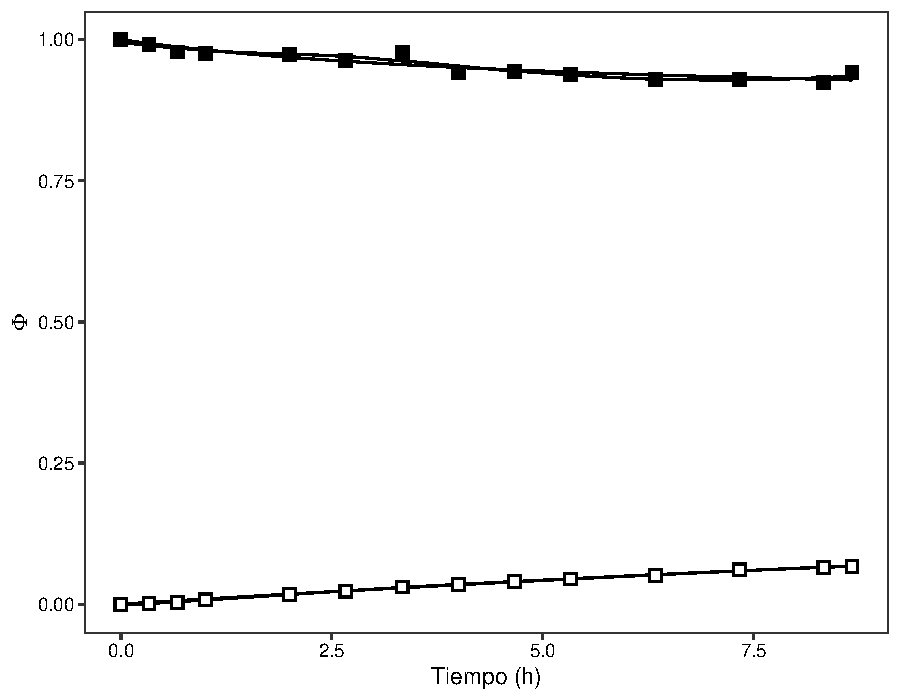
\includegraphics[height=0.388\textwidth]{chap5/figures/C1-profile.pdf}}
               \put(219, 168){\large a)}
               \end{picture}}%
    \subbottom{\begin{picture}(230,178)
               \put(0, 0){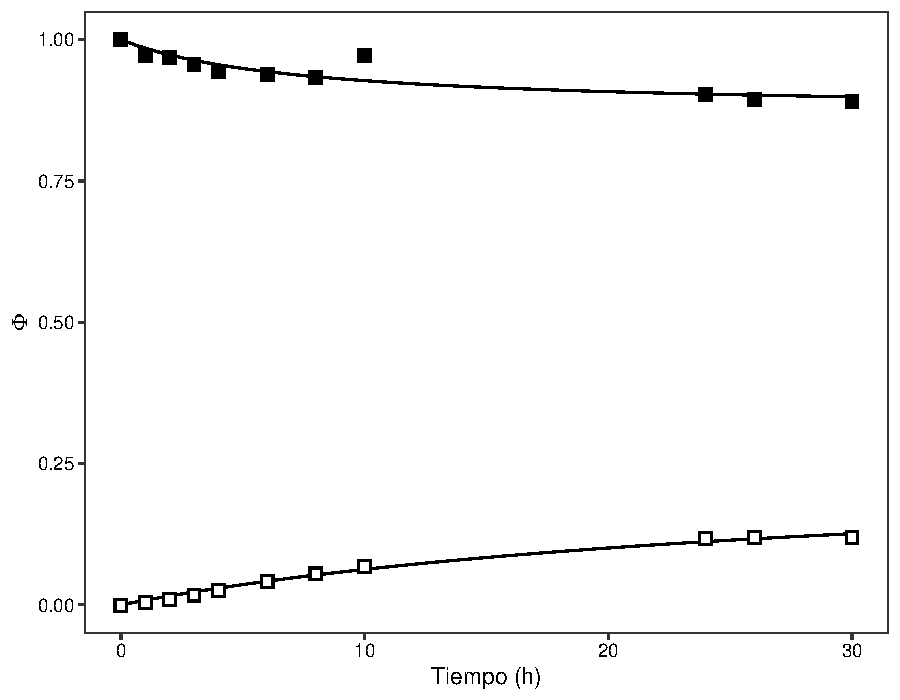
\includegraphics[height=0.388\textwidth, trim = {1.258cm 0 0 0},   clip]{chap5/figures/C2-profile.pdf}}
               \put(199, 168){\large b)}
               \end{picture}}
    \caption[Primeros perfiles de transporte de litio en celda de permeación.]{Perfiles de transporte de litio para las membranas C.1 y C.2. Litio en la fase de alimentación (\protect\squareblck) y litio en la fase de recuperación (\protect\squarewht).}        
    \label{fig:profileC1}
\end{figure}

\subsection{Primer diseño factorial fraccionado}\label{sec:FrF2-1}\index{Diseño de experimentos!factorial fraccionado}
Con el primer diseño experimental se pretendía encontrar el efecto a gran escala de la composición de la membrana y de las disoluciones de alimentación y de recuperación sobre la eficiencia del proceso de transporte. Se planteó una matriz de diseño factorial fraccionada de siete varia\-bles a dos niveles con resolución III. Las variables consideradas fueron las masas de polímero base (\textbf{X1}), plastificante (\textbf{X2}) y extractantes (\textbf{X3} y \textbf{X4} para LIX-54-100 y Cyanex~923, respectivamente) en la composición de la PIM, la concentración de hidróxido de sodio y de iones litio en la disolución de alimentación (\textbf{X5} y \textbf{X6}, respectivamente) y concentración de ácido clorhídrico en la fase de recuperación (\textbf{X7}). La respuesta (\textbf{Y}) fue la eficiencia del proceso de transporte de litio. La matriz de diseño y las respuestas de cada sistema se muestran en la Tabla \ref{tab:frf2matrix1}.  El diseño experimental fue creado y analizado usando el paquete \verb|FrF2| \citep{FrF2} de \verb|R-CRAN|.

\begin{table}[H]
    \centering\footnotesize
    \begin{tabular}{@{}ccccccccr@{}}\toprule
        \textbf{ID}& \textbf{X1} (mg)& \textbf{X2} (mg)& \textbf{X3} (mg)& \textbf{X4} (mg)& \textbf{X5} (mol~kg$^{-1}$)& \textbf{X6} (mg~kg\mnn)& \textbf{X7} (mol~kg\mnn) & \textbf{Y} (\%)\\\midrule
        D.1&30&   20&  12&     50&  0.001&    2&   0.1&2.4\\
        D.2&80&   20&  50&     12&  0.001&    2&   0.5&2.7\\
        \textbf{D.3}&\textbf{30}&   \textbf{40}&  \textbf{50}&     \textbf{12}&   \textbf{0.01}&    \textbf{2}&   \textbf{0.1}&\textbf{88.8}\\
        D.4&80&   20&  12&     12&   0.01&   10&   0.1&0.3\\
        D.5&80&   40&  50&     50&  0.001&   10&   0.1&0.0\\
        D.6&80&   40&  12&     50&   0.01&    2&   0.5&1.4\\
        D.7&30&   40&  12&     12&  0.001&   10&   0.5&0.3\\
        \textbf{D.8}&\textbf{30}&   \textbf{20}&  \textbf{50}&     \textbf{50}&   \textbf{0.01}&   \textbf{10}&   \textbf{0.5}&\textbf{22.2}\\\bottomrule
    \end{tabular}
    \caption{Matriz de diseño del primer diseño experimental factorial fraccionado.}
    \label{tab:frf2matrix1}
\end{table}


\begin{figure}[H]
    \centering
    \subbottom{\begin{picture}(245,178)
               \put(0, 0){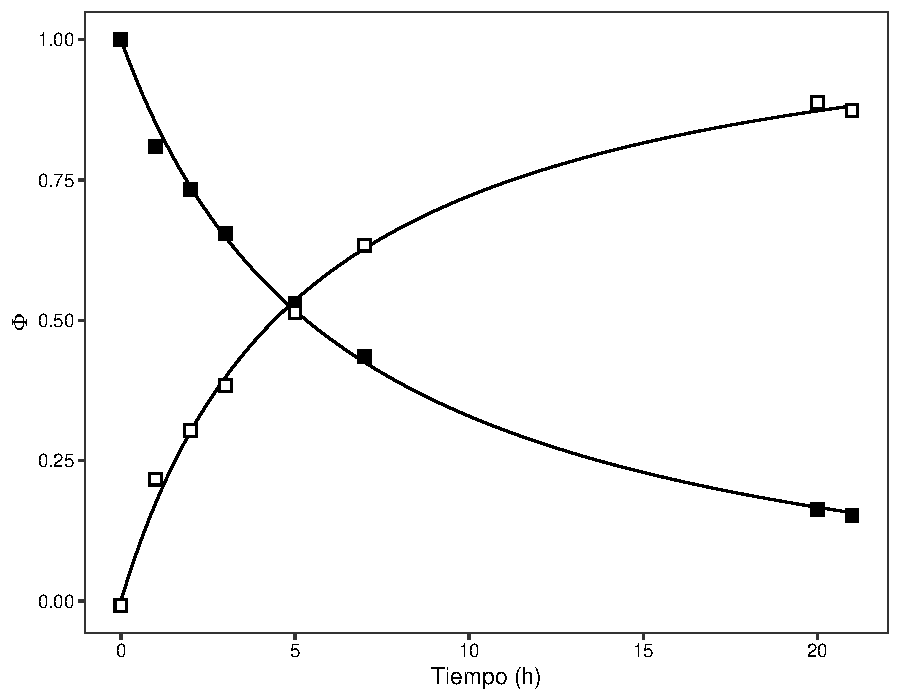
\includegraphics[height=0.388\textwidth]{chap5/figures/D3-profile.pdf}}
               \put(219, 167){\large a)}
               \end{picture}}%
    \subbottom{\begin{picture}(230,178)
               \put(0, 0){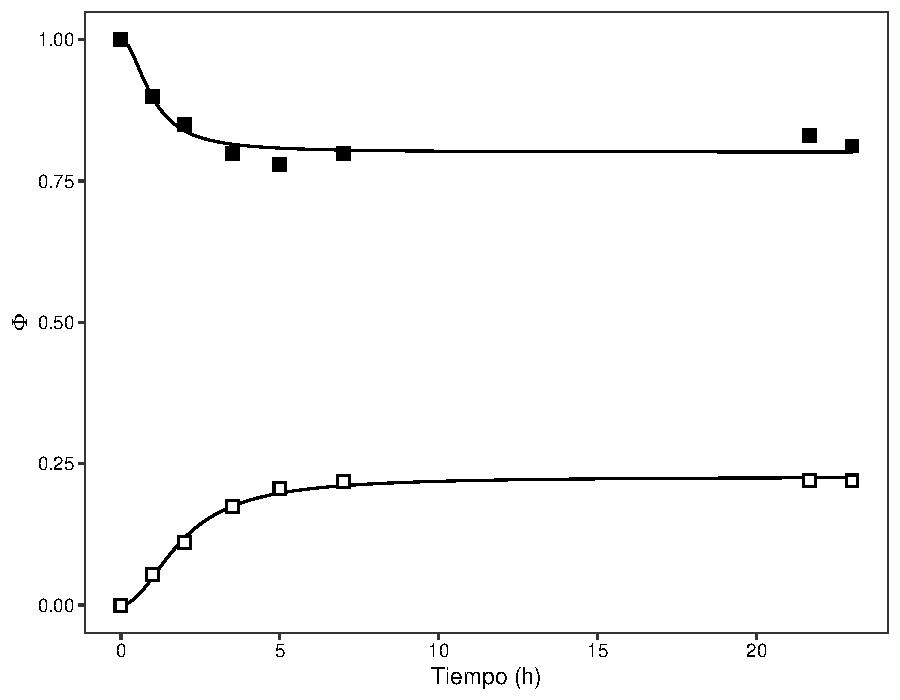
\includegraphics[height=0.388\textwidth, trim = {1.258cm 0 0 0},   clip]{chap5/figures/D8-profile.pdf}}
               \put(198, 167){\large b)}
               \end{picture}}
    \caption[Perfiles de transporte de litio membranas primer diseño factorial fraccionado.]{Perfiles de transporte de litio de los puntos 3 (a) y 8 (b) del primer diseño factorial fraccionado. Litio en la fase de alimentación (\protect\squareblck) y litio en la fase de recuperación (\protect\squarewht).}        
    \label{fig:FrF2_1.profiles}
\end{figure}

En la mayoría de los experimentos no se observa un transporte apreciable de litio hacia la diso\-lución de recuperación. Los perfiles de transporte de los únicos experimentos donde el litio fue transportado (PIM D.3 y PIM D.8) se muestran en la Figura \ref{fig:FrF2_1.profiles}. En el sistema que usa la PIM D.3 se observa que a las cinco horas de transporte el litio se encuentra a concentraciones iguales en ambas disoluciones y su transporte empieza a ocurrir en contra del gradiente de concentración. Este fue un avance importante en el desarrollo del método, dado que hasta el momento no se había observado el transporte activo del catión litio.

La respuesta de los experimentos es en general bastante mala, y como se observa en el gráfico de efectos principales (Figura \ref{fig:FrF2-ME.1}), no hay motivos para suponer la escasez de efectos, por lo que los diagramas de Daniel pueden no ser los más apropiados. No se dispone de un estimador independiente de la variabilidad del método y esto imposibilita el uso de otras herramientas, como el diagrama de Pareto. Bajo estas condiciones se dificulta mucho el análisis de los resultados del diseño por medio de herramientas {tradicionales} y puede concluirse que ninguna variable tiene un efecto importante en la respuesta del sistema dentro del intervalo de valores probados o bien, más probablemente, que la mayoría de las variables tienen una influencia significativa en el sistema. En diseños experimentales de cribado resulta peor ignorar la importancia de variables con efectos significativos que considerar como significativas a algunas variables no importantes \citep{FrF2}. Con base en esto, se decide analizar el gráfico de efectos principales en el modelo sin reducir.

\begin{figure}[H]
    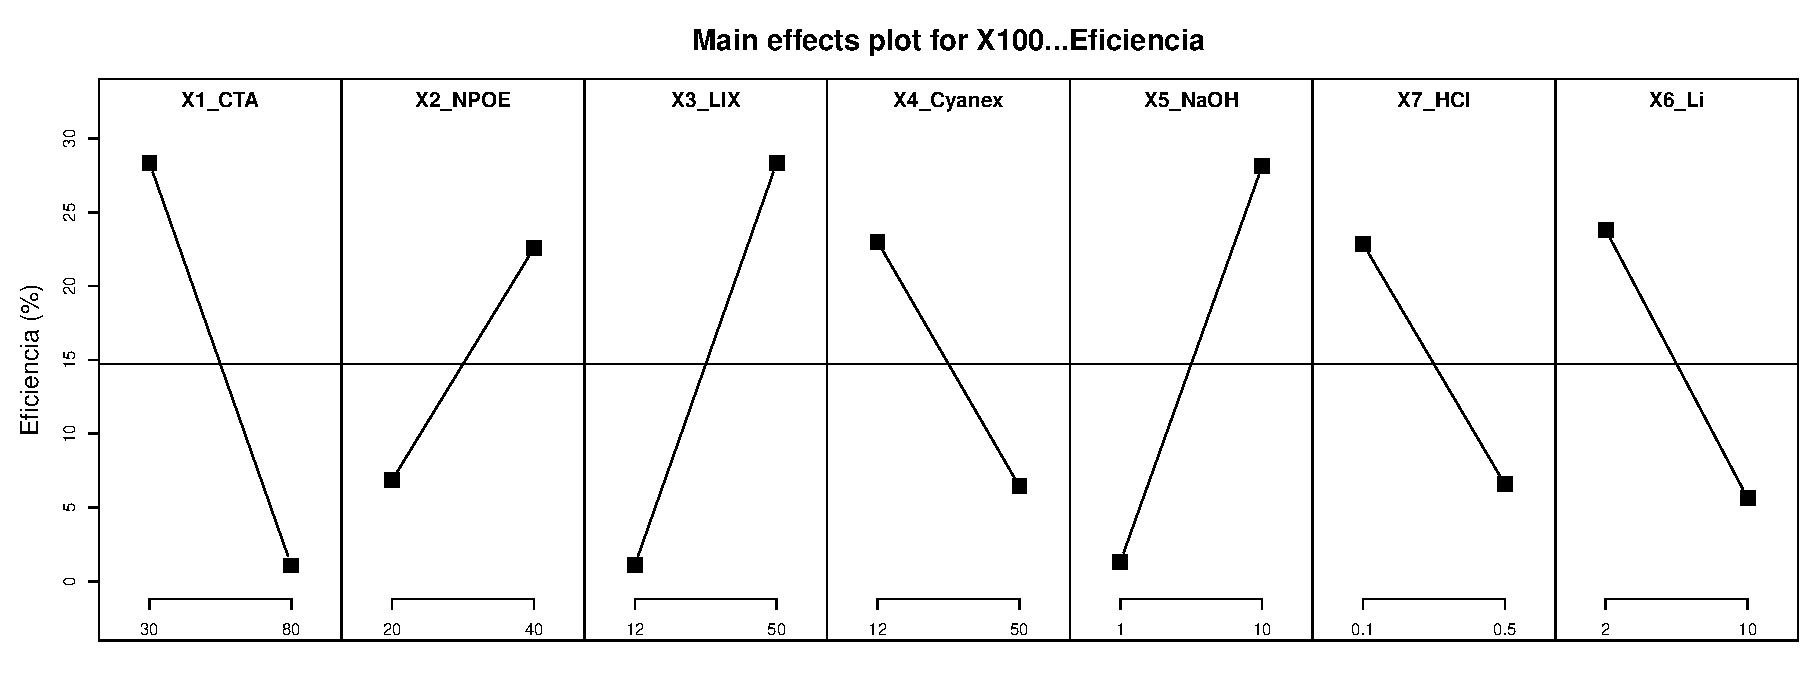
\includegraphics[width=\textwidth, trim = {0 1cm 0 1.34cm}, clip]{chap5/figures/MEP1.pdf}
    \caption[Gráfico de efectos principales del primer diseño factorial fraccionado.]{Gráfico de efectos principales del primer diseño factorial fraccionado. El eje de las abscisas que corresponde a la variable X5 (Concentración de hidróxido de sodio) ha sido multiplicado por 1000 para facilitar su visualización.}
    \label{fig:FrF2-ME.1}
\end{figure}

Los efectos de las variables son relativamente homogéneos, pero destacan ligeramente las masas de CTA y de LIX-54-100 en la membrana y la concentración inicial de hidróxido de sodio en la disolución de alimentación. Usando el método descrito en la Sección \ref{app:ParedesMethod}, el análisis de varianza de los modelos lineales simplificados univariados propuestos presentan \textit{valores p}  cercanos a 0.24 para las variables mencionadas. Esto indica que se carece de evidencia suficiente (con un 90\% de confianza) para aseverar que el efecto de modificar dichas variables en el intervalo considerado pueda distinguirse de la variabilidad propia del método. El resultado es similar cuando se analizan los modelos con las posibles combinaciones entre estas variables (por parejas y en terna) y carece de sentido intentar con las otras cuatro variables que presentan efectos principales inferiores en magnitud. 

Los resultados del diseño experimental no son suficientes para asegurar que el efecto de alguna variable en la eficiencia del sistema para extraer litio sea estadísticamente significativo. Debe tener\-se en cuenta que dicha conclusión está fuertemente influenciada por el hecho de que la mayo\-ría de las condiciones propuestas condujeron a procesos de transporte fallidos. Sin embargo, definitivamente algunas combinaciones de estas variables dan lugar a procesos de transporte significativamente mejores que algunas otras. El diagrama de efectos principales sugiere que un mejor transporte de iones litio se obtiene con una membrana de 30~mg de CTA, 40~mg de NPOE, 50~mg de LIX-54-100 y 12~mg de Cyanex~923, una disolución de alimentación de hidróxido de sodio 0.01~mol~kg\mnn\ y litio 2~mg~kg\mnn\ y una disolución de recuperación de ácido clorhídrico 0.1~mol~kg\mnn. Con base en esto, debe modificarse la metodología de análisis de los resultados y se considerará, simplemente, las condiciones bajo las cuales el transporte de litio fue posible a una escala apreciable (PIM D.3 y PIM D.8). 

Los sistemas PIM D.3 y PIM D.8 coinciden en que sus membranas contenían 30~mg de polímero base, 50~mg de LIX-54-100, y 0.01~mol~kg\mnn de hidróxido de sodio inicialmente en la fase de alimentación. El transporte es más eficiente cuando la concentración inicial de litio en la disolución de alimentación es pequeña, pues una menor cantidad de litio debe ser transportada a través de la membrana y la fracción transportada es mayor a tiempos menores. Una concentración inicial de litio en la fase de alimentación de 2~mg~kg\mnn\ presenta una ventaja adicional dado que, como se menciona en la Sección Anexa \ref{sec:liexternal}, la curva de calibración con patrones externos para litio por \ac{FAAS} presenta una buena linealidad hasta concentraciones de 2.5~mg~kg\mnn. Esto implica que si la disolución de alimentación contiene inicialmente 2~mg~kg\mnn\ de iones litio, no es necesario hacer diluciones para cuantificarlo. Las diluciones devengan tiempo valioso e introducen variación indeseada en los resultados para cuantificar la especie de interés. 

Respecto a la masa del extractante Cyanex~923, se observó que la elección de las variables \textbf{X3} y \textbf{X4} no fue la mas apropiada. Escoger la masa de cada extractante individualmente condujo a varias configuraciones en las que la relación molar entre estas especies era tan grande como 5.9:1 y tan pequeña como 0.34:1. Estos valores se encuentran muy alejados del reportado como óptimo por \citet{Pranolo2015}, y habría sido más conveniente utilizar como variables la masa total de extractantes y la relación molar entre estos. El perfil de transporte de la Figura \ref{fig:FrF2_1.profiles}(a)  sugiere que una masa de 12~mg de Cyanex~923 en la membrana produce transportes más eficientes, pero si se observa con detalle el sistema con la PIM D.8, se encuentra que la configuración que contiene 100~mg de extractantes en relación molar 1.41:1 transporta una cantidad neta de litio mucho mayor en tiempos más cortos. Este valor  de relación molar es similar al reportado por \citet{Pranolo2015}. Se sugiere que la relación molar óptima para el recobro de litio usando la PIM puede estar muy cerca de la reportada para el recobro de litio por \ac{SSX}.

Sobre la cantidad de plastificante en la membrana o la concentración inicial de ácido clorhídrico en la disolución de recuperación, no hay indicios que sugieran que un valor es mejor que el otro pero debió tomarse una decisión y con base en los buenos resultados del sistema PIM D.3 se escogieron 40~mg y 0.10~mol~kg\mnn, respectivamente.

Con base en lo discutido, se propuso una membrana con 30~mg de CTA, 40~mg de plastificante y 100~mg de una mezcla de extractantes LIX-54-100/Cyanex~923 en una relación molar 2:1. La concentración de hidróxido de sodio en la disolución de alimentación y de ácido clorhídrico en la disolución de recuperación para experimentos posteriores se fija en 0.01 y 0.1~mol~kg\mnn\, res\-pec\-tivamente. La concentración inicial de litio en las disoluciones de alimentación posteriores se mantuvo constante en 2~mg~kg\mnn.

\subsection{Efecto del plastificante en la eficiencia del transporte}\index{PIM!efecto del plastificante}
Las membranas preparadas hasta el momento han contenido siempre \ac{NPOE} como plastificante. La naturaleza del plastificante promueve modificaciones estructurales en la membrana y esto afecta el transporte de los iones a través de la misma \citep{RodriguezdeSanMiguel2008}. En busca de una membrana capaz de transportar litio con una mayor rapidez, se compararon formulaciones con los plastificantes \ac{NPOE}, tris(2-etilhexil)fosfato (TEHP)\acused{TEHP}, tris(2-butoxietil)fosfato (TBEP) \acused{TBEP} y sin plastificante (membranas E.1, E.2, E.3 y E.4, respectivamente). La composición de las membranas y de las disoluciones empleadas fue la descrita al final de la sección anterior. Los perfiles de transporte obtenidos se muestran en la Figura \ref{fig:plasti1}.

\begin{figure}[htbp]
    \centering
    \subbottom{\begin{picture}(245,160)
               \put(0, 0){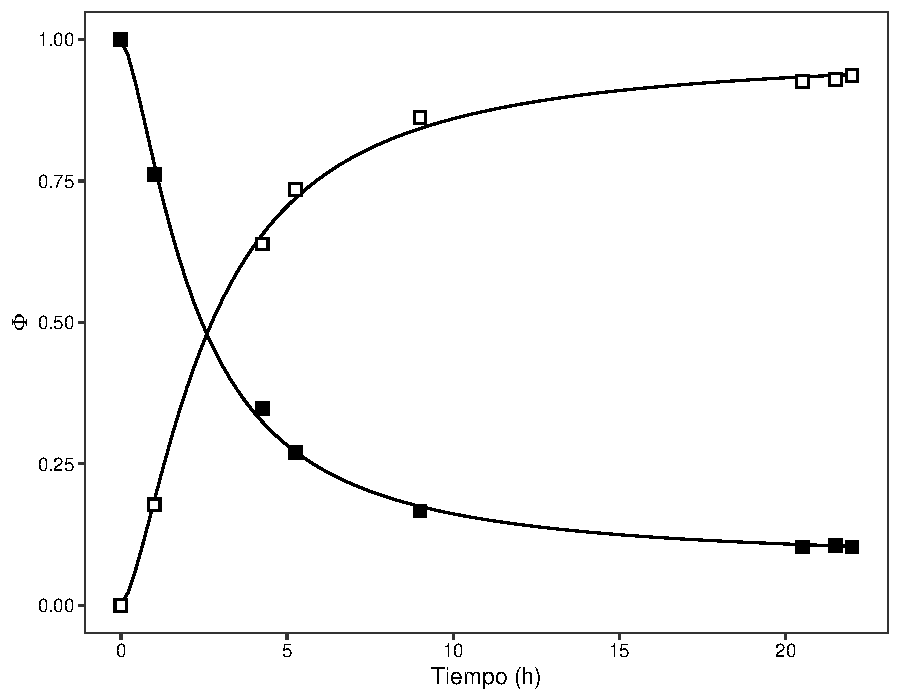
\includegraphics[height=0.355\textwidth, trim = {0 1cm 0 0},   clip]{chap5/figures/E.1-profile.pdf}}
               \put(218, 151.5){\large a)}
               \end{picture}}%
    \subbottom{\begin{picture}(230,160)
               \put(0, 0){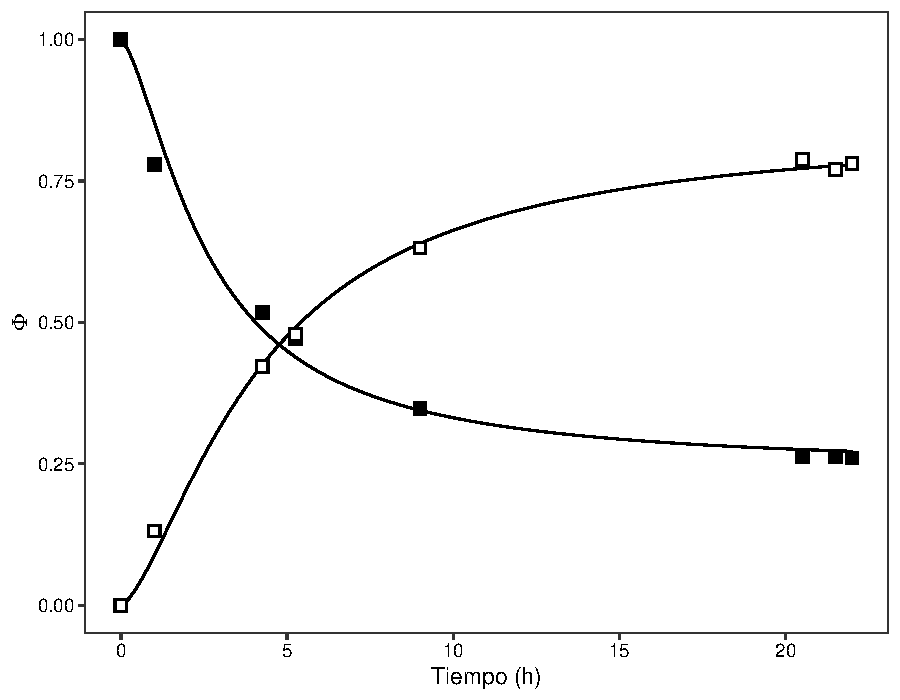
\includegraphics[height=0.355\textwidth, trim = {1.258cm 1cm 0 0},   clip]{chap5/figures/E.2-profile.pdf}}
               \put(197, 151.5){\large b)}
               \end{picture}}\\
    \subbottom{\begin{picture}(245,178)
               \put(0, 0){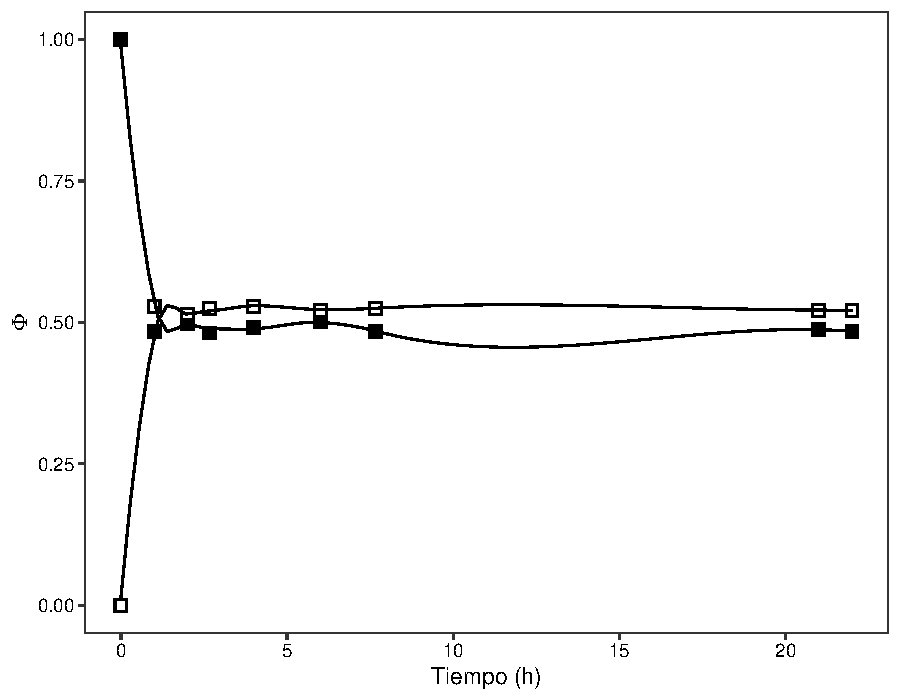
\includegraphics[height=0.388\textwidth]{chap5/figures/E.3-profile.pdf}}
               \put(218, 167){\large c)}
               \end{picture}}%
    \subbottom{\begin{picture}(230,178)
               \put(0, 0){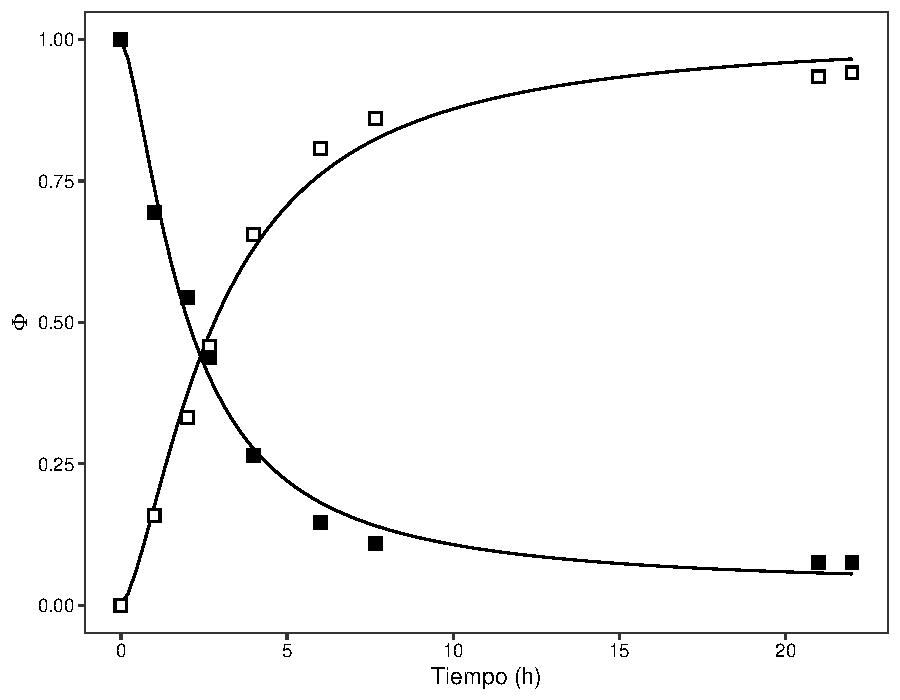
\includegraphics[height=0.388\textwidth, trim = {1.258cm 0 0 0},   clip]{chap5/figures/E.4-profile.pdf}}
               \put(197, 167){\large d)}
               \end{picture}}
    \caption[Perfiles de transporte de litio en membranas con distintos plastificantes.]{Perfiles de transporte de litio usando membranas sin plastificante (a), con NPOE (b), TEHP (c) y TBEP (d). Litio en la fase de alimentación (\protect\squareblck) y litio en la fase de recuperación (\protect\squarewht).}
    \label{fig:plasti1}
\end{figure}

La PIM que contiene \ac{TEHP} como plastificante posee pésimas propiedades mecánicas y se presentó una ruptura en la membrana. Las disoluciones de alimentación y de recuperación de este sistema se mezclaron y homogeneizaron como consecuencia de la agitación de las semiceldas. No fue posible observar transporte de litio mediado por la PIM. La concentración de litio en la disolución de recuperación para tiempos distintos de cero parece mayor a la determinada en la disolución de alimentación, pero esta diferencia no es importante y corresponde a que se usaron distintas curvas de calibración para compensar el efecto matriz en la cuantificación (ver Sección Anexa \ref{sec:liexternal}). 

La membrana sin plastificante presenta excelente desempeño. La eficiencia obtenida en el transporte de litio es del 94\%. Un desempeño similar se observa para la PIM con TBEP como plastificante en su composición. El NPOE confiere propiedades mecánicas aceptables a la membrana pero el desempeño de la misma es inferior respecto a las PIMs con TBEP o sin plastificante. Las propiedades mecánicas de la membrana sin plastificante fueron en general bastante buenas.

La principal función del plastificante en una PIM es mejorar su resistencia mecánica y su flexibilidad. Esto se logra por medio de la disminución de fuerzas intermoleculares entre las cadenas del polímero base. Una distancias media más grande entre las cadenas poliméricas ocasiona el ensanchamiento de la membrana \citep{Witt2018}. No incluir un plastificante adicional en la membrana evita un aumento en su grosor. Una membrana más delgada favorece el transporte de litio a través de la misma. La fabricación de PIMs sin plastificante que presentan buenas propiedades mecánicas y un buen desempeño para el transporte de diversas especies ha sido reportada por varios autores \citep{Vazquez2014, Xiong2019}. En estos casos, el extractante presenta doble función de extractante y plastificante.

%Entre los dos extractantes presentes en la PIM, el Cyanex~923 es probablemente el que hace también de plastificante. Distintos ésteres de ácido fosfórico han sido reportados como plastificantes de uso común en varios polímeros de uso industrial \citep{Wypych2017} pero no se encontraron reportes de óxidos de alquilfosfina usados para tal fin. \citet{Mead1942} reportaron que el tamaño y la forma de los plastificantes tiene una mayor influencia en su capacidad para plastificar que las particularidades de su estructura química. Los óxidos de alquilfosfinas tienen casi la misma cabeza polar que los ésteres de ácido fosfórico y esto los haría, \textit{grosso modo,} equivalentes como plastificantes a los esteres de ácido fosfórico con sustituyentes similares. Moléculas con cadenas alifáticas lineales (entre seis y ocho átomos de carbono para el caso del Cyanex~923) tienen mejores propiedades como plastificantes que moléculas con grupos cíclicos voluminosos (fenil en el caso del LIX-54-100) \citep{Mead1942}.

Un componente menos en la formulación de la PIM implica una variable menos que debe ser estudiada y optimizada. Esto a la vez se traduce en un costo de producción inferior que puede hacer más atractivo el escalamiento de la tecnología para una eventual aplicación industrial.
%\subsubsection{Primera optimización simplex}\label{sec:smplxexperimental1}
%Se buscó una mejora en el proceso de transporte por medio de una optimización siguiendo el algoritmo simplex modificado. Tras decidir que la membrana no llevaría plastificante en su composición (ver Sección \ref{sec:plasti1}), las variables consideradas fueron las masas de polímero base (\textbf{X1}) y de mezcla de extractantes (\textbf{X2}), la relación molar Lix-54-100/Cyanex923 en la mezcla (\textbf{X3}) y las concentraciones de hidróxido de sodio en la disolución de alimentación (\textbf{X4}) y de ácido clorhídrico en la disolución de recuperación. La variable respuesta ($\Upsilon$) se muestra en la ecuación \ref{ec:varUpsilon1}. 

%\begin{equation}\label{ec:varUpsilon1}
%    \Upsilon_i = \overline{\alpha_i}\cdot\overline{\beta_i}^{-1}
%\end{equation}
%donde $\overline{\alpha_i}$ y $\overline{\beta_i}$ son los parámetros de regresión (combinados) de la Ecuación \ref{eq:NLSCRIS} que describe los perfiles de transporte obtenidos en el \textit{i-}ésimo experimento (ver Sección \ref{sec:NLS}).

%El proceso de optimización se llevó a cabo con la ayuda del paquete \verb|labsimplex| del programa estadístico R  \citep{labsimplex}. Las coordenadas del punto inicial, el tamaño de paso y las coordenadas de los vértices del primer simplex se muestran en la Tabla \ref{tab:smplx1.1}.
%\begin{table}[H]
%    \centering\footnotesize
%    \begin{tabular}{@{}lccccc@{}}\toprule
%        \textbf{ID} & \textbf{X1} (mg) & \textbf{X2} (mg) & \textbf{X3} & \textbf{X4} (mol~kg\mnn\) & \textbf{X5} (mol~kg\mnn\) \\\midrule
%        \textit{Punto inicial} & 30 & 100 & 2.00 & 0.010 & 0.100\\
%        \textit{Tamaño de paso}& 10 &  20 & 1.00 & 0.005 & 0.050\\\midrule
%        F.1 \textit{(Vértice 1)}& 30&  100&    2.00& 0.010& 0.100\\
%        F.2 \textit{(Vértice 2)}&  40&   84&    2.00& 0.010& 0.100\\
%        F.3 \textit{(Vértice 3)}&  40&  104&    2.75& 0.010& 0.100\\
%        F.4 \textit{(Vértice 4)}&  40&  104&    1.75& 0.013& 0.100\\
%        F.5 \textit{(Vértice 5)}&  40&  104&    1.75& 0.008& 0.124\\
%        F.6 \textit{(Vértice 6)}&  40&  104&    1.75& 0.008& 0.074\\\bottomrule
%    \end{tabular}
%    \caption{Configuración y coordenadas del simplex de la primera optimización.}
%    \label{tab:smplx1.1}
%\end{table}

\subsection{Cambio de la base en la disolución de alimentación}
En el proceso de mejora de las condiciones para la extracción de litio se ha observado un dete\-rioro en la selectividad del sistema conforme se plantean condiciones que conducen a transportes más eficientes. Los iones sodio provenientes del hidróxido de sodio que se usa para alcalinizar la disolución de alimentación han sido identificados en la fase de recuperación cuando se cuantifica litio por \ac{FAAS}. Se observó que hasta un 25\% del sodio inicialmente presente en la disolución de alimentación puede ser cotransportado junto con el ion litio, y se decidió que era importante monitorear su proceso de transporte. 
%\begin{wrapfigure}{r}{0.55\textwidth}
%  \centering
%  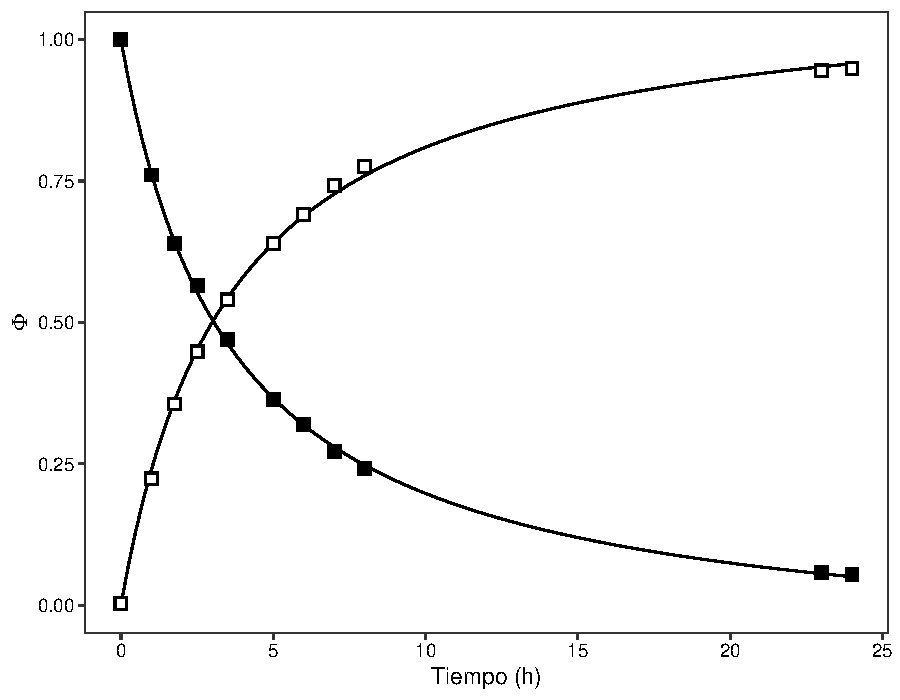
\includegraphics[height=0.388\textwidth]{chap5/figures/g1profile.pdf}
%  \caption{\vspace{-1ex}Perfil de transporte de litio usando hidróxido de amonio en la fase de alimentación.}
%  \label{fig:amonio1}
%\end{wrapfigure}

Se probó el reemplazo del hidróxido de sodio por hidróxido de amonio en la fase de alimentación para eliminar la omnipresencia de los iones sodio en todas las disoluciones de alimentación. Esto permitió estudiar el proceso de transporte cuando el litio es el único catión metálico en la fase de alimentación y permitió modificar sistemáticamente la concentración de los iones interferentes en esta disolución con el fin de facilitar el estudio de la selectividad de los sistemas. 

El perfil de transporte obtenido usando hidróxido de amonio 0.012~mol~kg\mnn\ en la fase de alimentación se muestra en la Figura \ref{fig:amonio1}. Puede observarse que la eficiencia en el transporte no disminuye como consecuencia del cambio de base, pero la velocidad a la que el litio es transportado a la fase de recuperación es menor que cuando se usa una base fuerte (hidróxido de sodio).
\begin{figure}[H]
  \centering
  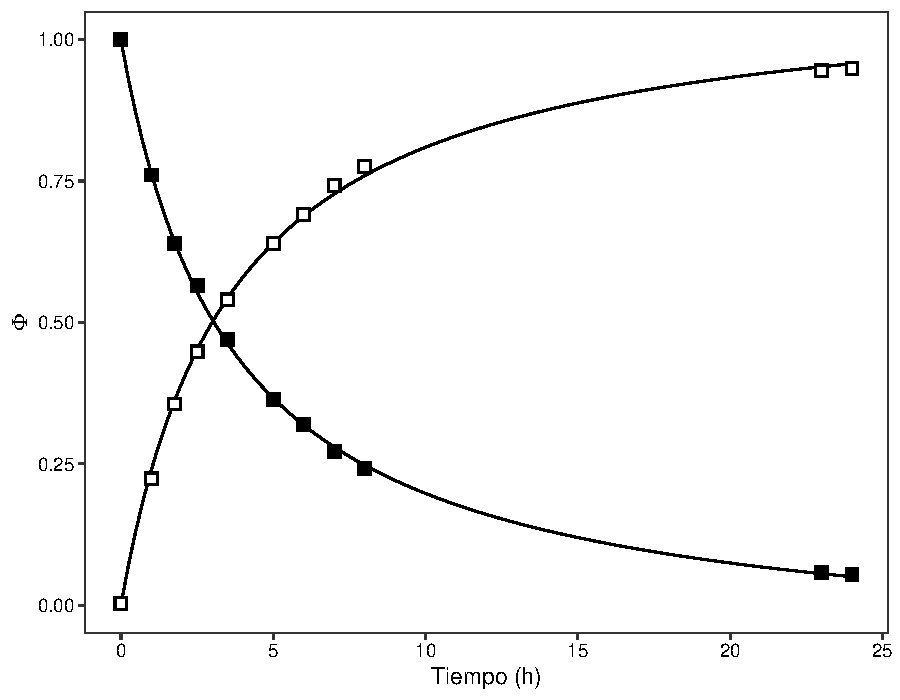
\includegraphics[height=0.388\textwidth]{chap5/figures/g1profile.pdf}
  \caption[Perfil de transporte de litio usando hidróxido de amonio en la fase de alimentación.]{Perfil de transporte de litio usando hidróxido de amonio en la fase de alimentación. Litio en la fase de alimentación (\protect\squareblck) y litio en la fase de recuperación (\protect\squarewht).}
  \label{fig:amonio1}
\end{figure}


\subsection{Segundo diseño factorial fraccionado}\index{Diseño de experimentos!factorial fraccionado}
En un nuevo diseño factorial fraccionado se pretendió encontrar condiciones para un transporte más rápido y eficiente, controlando la selectividad del sistema. Considerando la experiencia adquirida del diseño anterior, se escogieron las variables masa de polímero base (\textbf{X1}), masa de mezcla de extractantes (\textbf{X2}), relación molar LIX-54-100/Cyanex~923 en la mezcla de extractantes (\textbf{X3}) y las concentraciones de hidróxido de amonio en la disolución de alimentación (\textbf{X4}) y de ácido clorhídrico en la disolución de recuperación (\textbf{X5}). La matriz de diseño generada con el paquete \verb|FrF2| \citep{FrF2} se muestra en la Tabla \ref{tab:frf2matrix2}.

\begin{table}[H]
    \centering\footnotesize
    \begin{tabular}{@{}lccccc@{}}\toprule
        \textbf{ID}& \textbf{X1} (mg)& \textbf{X2} (mg)& \textbf{X3}& \textbf{X4} (mol~kg\mnn)& \textbf{X5} (mol~kg\mnn)
        \\\midrule
       H.1 & 30 &  70  &  2.0&    0.02 & 0.04\\
       H.2 & 45 &  70  &  3.5&    0.01 & 0.04\\
       H.3 & 30 & 110  &  3.5&    0.01 & 0.07\\
       H.4 & 45 &  70  &  2.0&    0.01 & 0.07\\
       H.5 & 45 & 110  &  3.5&    0.02 & 0.04\\
       H.6 & 45 & 110  &  2.0&    0.02 & 0.07\\
       H.7 & 30 & 110  &  2.0&    0.01 & 0.04\\
       H.8 & 30 &  70  &  3.5&    0.02 & 0.07\\\bottomrule
    \end{tabular}
    \caption{Matriz de diseño del segundo diseño experimental factorial fraccionado.}
    \label{tab:frf2matrix2}
\end{table}

Los procesos de transporte fueron monitoreados por 24 horas. La concentración de iones litio en la disolución de alimentación fue de 2~mg~kg\mnn. La selectividad de los sistemas fue evaluada respecto al transporte competitivo de iones sodio. Para esto, la disolución de alimentación contenía iones sodio en un exceso molar de 10:1 respecto al litio (concentración en masa iones sodio: 70~mg~kg\mnn). 

Se consideraron cuatro respuestas de manera independiente. Se tomaron los parámetros promediados $\alpha$ y $\beta$ de la regresión no lineal de los perfiles de transporte (Ecuación \ref{eq:NLSCRIS} de la Sección \ref{sec:NLS}) y el valor máximo del factor de separación litio/sodio ($Sf_{\ce{Li}/\ce{Na}}$). Las tres respuestas mencionadas fueron combinadas por medio de una función de deseabilidad \citep{Derringer} y fue considerada como una cuarta respuesta ($D$) que se analizó independientemente con el propósito de averiguar si es posible resumir todas las respuestas simultáneamente sin perder información relevante.\index{Diseño de experimentos!función deseabilidad}

En todos los experimentos se observó un transporte apreciable de iones litio. Los resultados se resumen en la Tabla \ref{tab:frf2results2}. Contrario a lo presentado en el anterior diseño experimental fraccionado (Sección \ref{sec:FrF2-1}), la respuesta más uniforme en los experimentos del presente conjunto permite un análisis más robusto considerando la significancia estadística del efecto de cada variable. 
\begin{table}[H]
    \centering\footnotesize
    \begin{tabular}{@{}ccccc@{}}\toprule
        \textbf{ID} & $\overline{\alpha}$ & $\overline{\beta}$ & $F_{\ce{Li}/\ce{Na}}$&$D$\\\midrule
        H.1 & 1.05 $\pm$ 0.01   & 0.96 $\pm$ 0.06   & 46.6 &0.67\\
        H.2 & 0.83 $\pm$ 0.01   & 0.15 $\pm$ 0.01   & 32.6 &0.00\\
        H.3 & 0.79 $\pm$ 0.01   & 0.59 $\pm$ 0.03   & 23.2 &0.00\\
        H.4 & 1.08 $\pm$ 0.01   & 0.29 $\pm$ 0.01   & 56.2 &0.47\\
        H.5 & 1.06 $\pm$ 0.02   & 0.63 $\pm$ 0.04   & 67.6 &0.79\\
        H.6 & 1.07 $\pm$ 0.01   & 0.29 $\pm$ 0.01   & 74.5 &0.56\\
        H.7 & 1.05 $\pm$ 0.01   & 0.78 $\pm$ 0.05   & 36.3 &0.53\\
        H.8 & 1.05 $\pm$ 0.01   & 0.62 $\pm$ 0.03   & 62.5 &0.74\\\bottomrule
    \end{tabular}
    \caption{Resultados segundo diseño experimental fraccionado.}
    \label{tab:frf2results2}
\end{table}

Los diagramas de Daniel para las cuatro variables respuesta se muestran en la Figura \ref{fig:DanielFrF2-2}. Las variables con efectos estadísticamente significativos se marcaron haciendo uso del método numé\-rico de \citet{Lenth1989} implementado en el paquete \verb|FrF2|. En estos diagramas aparece el efecto de la interacción entre las variables \textbf{X2:X3} y \textbf{X2:X5}. Las demás interacciones no aparecen debido a la estructura alias usada para generar la matriz de diseño. Las otras interacciones entre variables son alias (i.e. coinciden los contrastes y son obtenidos en conjunto) de alguna de las variables consideradas independientemente.

\begin{figure}[H]
    \centering
    \subbottom{\begin{picture}(240,138)
               \put(0, 0){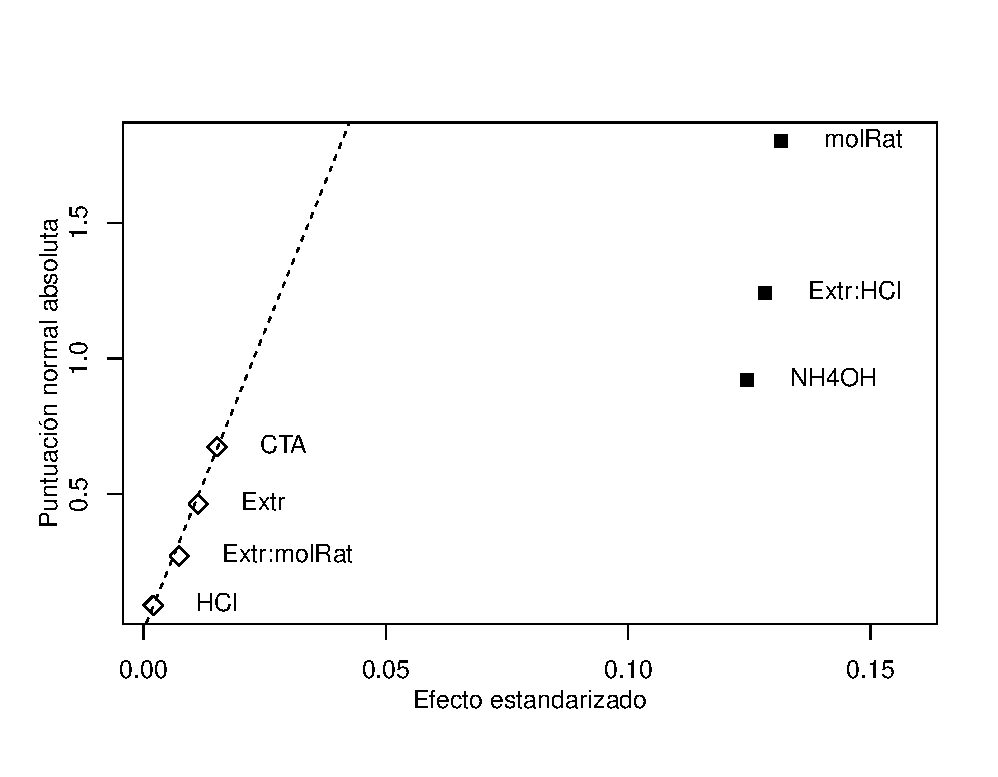
\includegraphics[height=0.355\textwidth, trim = {0 1.55cm 0 0},   clip, page = 1 ]{chap5/figures/DanielPlotsFrF2-2.pdf}}
               \put(32.8, 125){\large a)}
               \end{picture}}%
    \subbottom{\begin{picture}(230,138)
               \put(0, 0){\includegraphics[height=0.355\textwidth, trim = {1.92cm 1.55cm 0 0},   clip, page = 2 ]{chap5/figures/DanielPlotsFrF2-2.pdf}}
               \put(4.8, 125){\large b)}
               \end{picture}}\\
    \subbottom{\begin{picture}(240,138)
               \put(0, 0){\includegraphics[height=0.369\textwidth, page = 3, trim = {0 1.1cm 0 0},   clip ]{chap5/figures/DanielPlotsFrF2-2.pdf}}
               \put(32.8, 131){\large c)}
               \end{picture}}%
    \subbottom{\begin{picture}(230,138)
               \put(0, 0){\includegraphics[height=0.369\textwidth, trim = {1.92cm 1.1cm 0 0},   clip, page = 4 ]{chap5/figures/DanielPlotsFrF2-2.pdf}}
               \put(4.8, 131){\large d)}
               \end{picture}}
    \caption[Diagramas de Daniel del segundo diseño factorial fraccionado.]{Diagramas de Daniel del segundo diseño factorial fraccionado para las diferentes respuestas consideradas: Parámetro promediado $\alpha$ (a), parámetro promediado $\beta$ (b), coeficiente de separación (c) y función de deseabilidad (d). Variables con efectos estadísticamente significativos (\protect\squareblck) y variables cuyo efecto no puede diferenciarse del mero error aleatorio (\protect\squarerttdwht).}
    \label{fig:DanielFrF2-2}
\end{figure}

Puede observarse en la Figura \ref{fig:DanielFrF2-2}(d) que el análisis de los resultados a través de la función de deseabilidad logra resumir la mayoría de las conclusiones que pueden obtenerse considerando las variables respuesta cada una por separado. La única excepción se presenta con la variable de masa polímero base en la membrana (\textbf{X1}, CTA), que según la Figura \ref{fig:DanielFrF2-2}(b) tiene un efecto estadísticamente significativo sobre el parámetro $\beta$ que se relaciona con la rapidez a la que ocurre el proceso de transporte. El efecto de esta variable no ha resultado estadísticamente significativo cuando el análisis se hace usando la función deseabilidad.

El efecto de las variables que se han encontrado como estadísticamente significativas puede ser observado en un gráfico de efectos principales similar al mostrado en la Figura \ref{fig:FrF2-ME.1}. Sin embargo, dado que una de las interacciones que no poseen ningún alias ha sido marcada como importante según los diagramas de Daniel y el método de Lenth, es más apropiado visualizar los resultados en un gráfico de interacciones que permite el estudio los efectos principales proyectados en dos dimensiones que consideran los niveles de todas las variables combinadas entre sí. El gráfico de interacciones usando la función de deseabilidad como respuesta se muestra en la Figura \ref{fig:IAPLOTFrF2-2}. 

\begin{figure}[H]
    \centering
    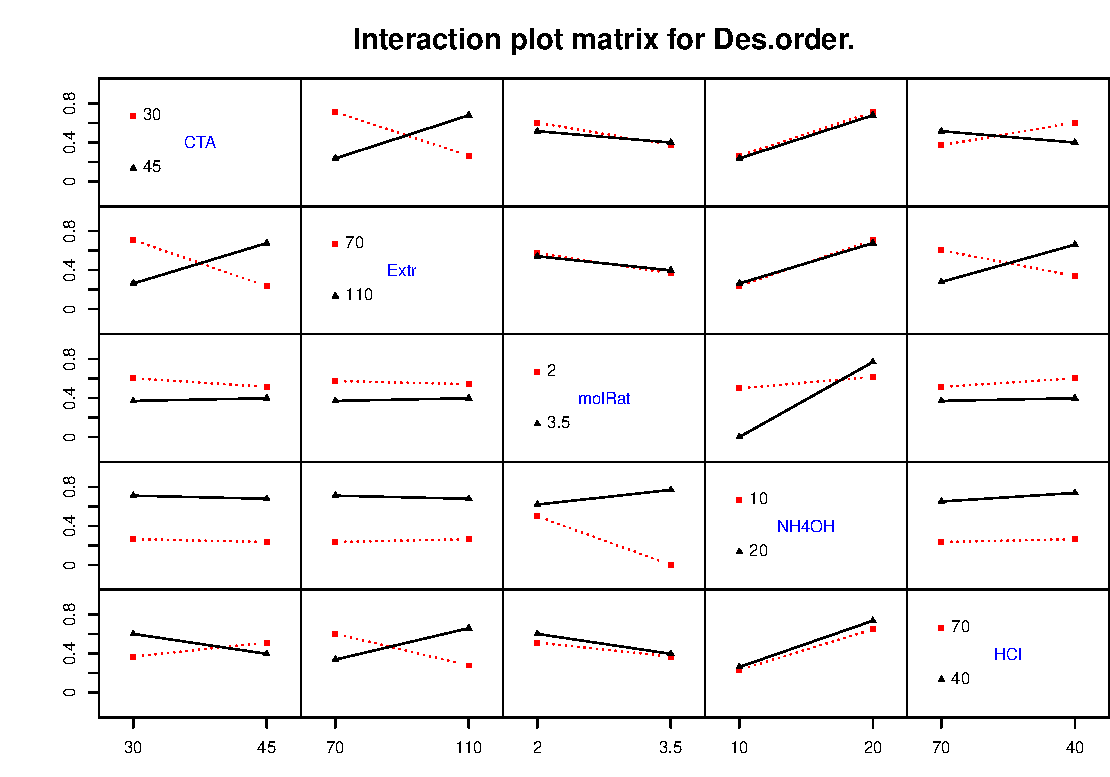
\includegraphics[width=0.9\textwidth, trim={1cm 0.3cm 0 1cm}, clip]{chap5/figures/IAPlotFrF2-2.pdf}
    \caption[Gráfico de interacciones del segundo diseño factorial fraccionado.]{Gráfico de interacciones de las variables consideradas en el segundo diseño factorial fraccionado. Los ejes de las abscisas que corresponden a las variables X4 y X5 (concentración de hidróxido de sodio y de ácido clorhídrico) han sido multiplicados por 1000 para facilitar su visualización.}
    \label{fig:IAPLOTFrF2-2}
\end{figure}

De la forma de las rectas de la Figura \ref{fig:IAPLOTFrF2-2}, considerando los diagramas de Daniel presentados anteriormente para tener en cuenta únicamente las variables cuyo efecto ha resultado estadísticamente significativo, se deduce lo siguiente:
\begin{itemize}
    \item Una concentración inicial de 0.02~mol~kg\mnn\ de hidróxido de amonio en la disolución de alimentación se traduce en procesos de transporte más eficientes y más selectivos.
    \item Los transportes son más eficientes usando membranas con una relación molar de extractantes LIX-54-100/Cyanex~923 de 2 que cuando se usa 3.5.
    \item Con el diagrama de efectos principales para la variable respuesta $\beta$ (no mostrado acá) se deduce que membranas con 30~mg de polímero base conducen a transportes más rápidos que cuando se usan 45~mg. Esto es lógico considerando que el grosor de la membrana está fuertemente influenciado por la cantidad de polímero base que lleva. Membranas más gruesas implican una región mayor del espacio que debe atravezar el litio para llegar a la fase de recuperación. Membranas con menos de 30~mg de CTA fueron preparadas para obtener transportes más rápidos, pero una cantidad de polímero base tan pequeña no provee del soporte y la resistencia mecánica suficiente para que la membrana resulte de alguna utilidad.
    \item El efecto de la masa total de extractantes en la membrana depende de la concentración inicial de ácido en la disolución de recuperación. Los transportes en los que se usan membranas con una masa de mezcla de extractantes pequeña (70~mg) son más eficientes si la concentración inicial de ácido en la disolución de recuperación es de 0.07~mol~kg\mnn\ (respecto a cuando se usa 0.04~mol~kg\mnn). Lo contrario se observa cuando se usan masas mayores de extractantes en la composición de la membrana.
\end{itemize}

La Tabla \ref{tab:paredesFrF2-2} contiene el resumen de los resultados obtenidos al usar el método propuesto descrito en la Sección \ref{app:ParedesMethod} para determinar que variables resultaron tener un efecto estadísticamente significativo sobre las cuatro respuestas consideradas. Los resultados del método se muestran como las variables cuyo valor p es inferior a la significancia escogida (0.10) en al menos uno de los análisis de varianza efectuados sobre los distintos modelos lineales que consideran un distinto número de variables explicatorias a la vez. El análisis se hace para cada respuesta con el fin de comparar las conclusiones que pueden obtenerse por este método con las obtenidas en párrafos anteriores.

\begin{table}[H]
    \centering\footnotesize
    \begin{tabular}{@{}llll@{}}\toprule
        \multirow{2}{*}{\textbf{Respuesta}} & \textbf{Numero de} & \textbf{Variables} & \multirow{2}{*}{\textbf{Valores P}} \\
        &\textbf{variables} &\textbf{significativas}\\\midrule
        Parámetro $\alpha$ & 1 & - & -\\
                           & 2 & X3, X4 & 0.07, 0.08\\
                           & 3 & - & -\\
                           & 4 & - & - \\
                           & 5 & - & - \\\midrule
        Parámetro $\beta$  & 1 & X1 & 0.02\\
                           & 2 & X1 & 0.03\\
                           & 3 & X1 & 0.05\\
                           & 4 & X1 & 0.06\\
                           & 5 & X1 & 0.06 \\\midrule
        Factor de separación & 1 & X4 & 0.03\\
                             & 2 & X4 & 0.05\\
                             & 3 & X1, X4 & 0.09, 0.07\\
                             & 4 & X1, X4 & 0.10, 0.06\\
                             & 5 & X4 & 0.09\\\midrule
        Función de deseabilidad & 1 & X4 & 0.03\\
                                & 2 & X4 & 0.04\\
                                & 3 & X4 & 0.07\\
                                & 4 & X4 & 0.06\\
                                & 5 & - & - \\\bottomrule
    \end{tabular}
    \caption[Variables con efectos estadísticamente significativos.]{Variables con efectos estadísticamente significativos según el nuevo método propuesto.}
    \label{tab:paredesFrF2-2}
\end{table}
No se incluyó la interacción entre pares de variables dado que la estructura alias de la matriz de diseño involucra la superposición de varios efectos individuales con la interacción entre varios pares de variables. Esto implica que varias interacciones entre parejas de variables pueden ser erróneamente interpretadas a menos que se trate de las variables \textbf{X2:X3} y \textbf{X2:X5} que se evaluaron en ausencia de la sobreposición de efectos de variables individuales. Esto presenta una posible pérdida valiosa de información que puede solucionarse si se incluyen solo las interacciones libres de estructuras alias, pero no se encontró una forma automática de hacer esto.

Las variables explicatorias que han resultado estadísticamente significativas para las distintas respuestas coinciden en su mayoría con las que han sido seleccionadas usando el diagrama de Daniel en conjunto con el método de Lenth. Las excepciones las presentan las variables respuesta \textit{selectividad} y \textit{función de deseabilidad}. Para la función de deseabilidad solo se ha identificado como relevante la concentración inicial de hidróxido de amonio en la disolución de alimentación mientras el efecto de la relación molar de los extractantes no ha podido ser diferenciado de la variación propia del método a un nivel de confianza del 90\%. Respecto a la selectividad del método, la masa de CTA en la membrana parece tener un efecto estadísticamente significativo que es contrario al encontrado para la velocidad del proceso (parámetro $\beta$). Probablemente, membranas más gruesas afectan en mayor proporción al transporte de cationes interferentes que al transporte de iones litio.

Con las conclusiones obtenidas se propone una composición de la \ac{PIM} con 30~mg de polímero base y 70~mg de mezcla de extractantes LIX-54-100/Cyanex~923 en relación molar 2:1, una concentración inicial de hidróxido de amonio en la disolución de alimentación de 0.02~mol~kg\mnn\ y una concentración inicial de ácido clorhídrico en la disolución de recuperación de 0.07~mol~kg\mnn.

\subsection{Condiciones hidrodinámicas y reproducibilidad}\label{sec:reprod}
Los perfiles de transporte de litio hacia la disolución de recuperación para distintos valores de rapidez de rotación de la propela en el compartimiento de la disolución de alimentación se muestran en la Figura \ref{fig:RPM1}(a). La fracción de litio transportada al final del proceso de transporte en función de la rapidez de rotación se muestra en la Figura \ref{fig:RPM1}(b). 

\begin{figure}[H]
    \centering
    \subbottom{\begin{picture}(240,167)
               \put(0, 0){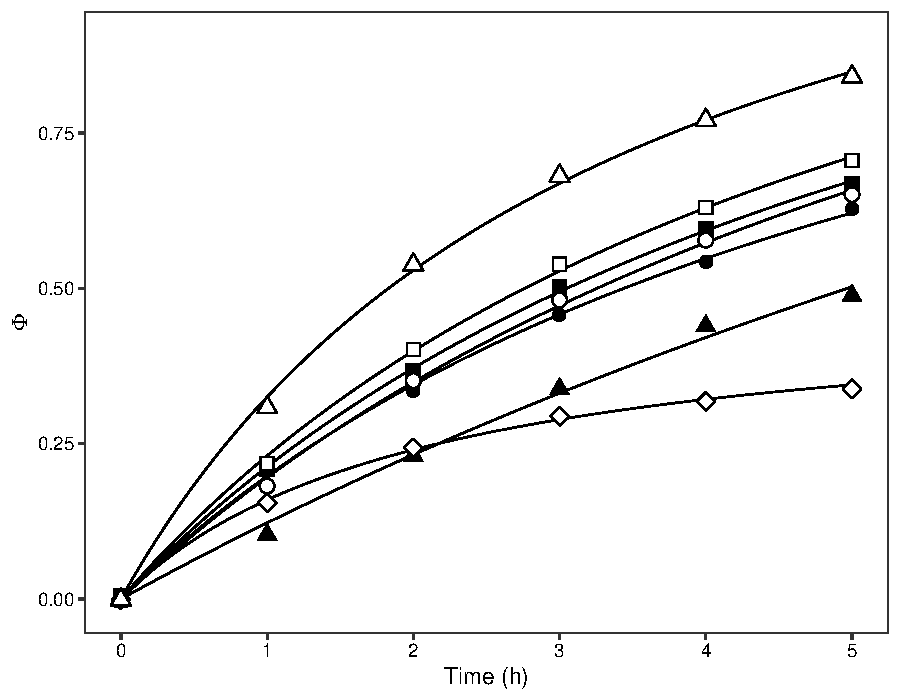
\includegraphics[height=0.375\textwidth, trim = {0 0 0 0},   clip]{chap5/figures/Thetha1_profiles.pdf}}
               \put(23, 160){\large a)}
                \end{picture}}%
    \subbottom{\begin{picture}(190,167)
               \put(0, 0){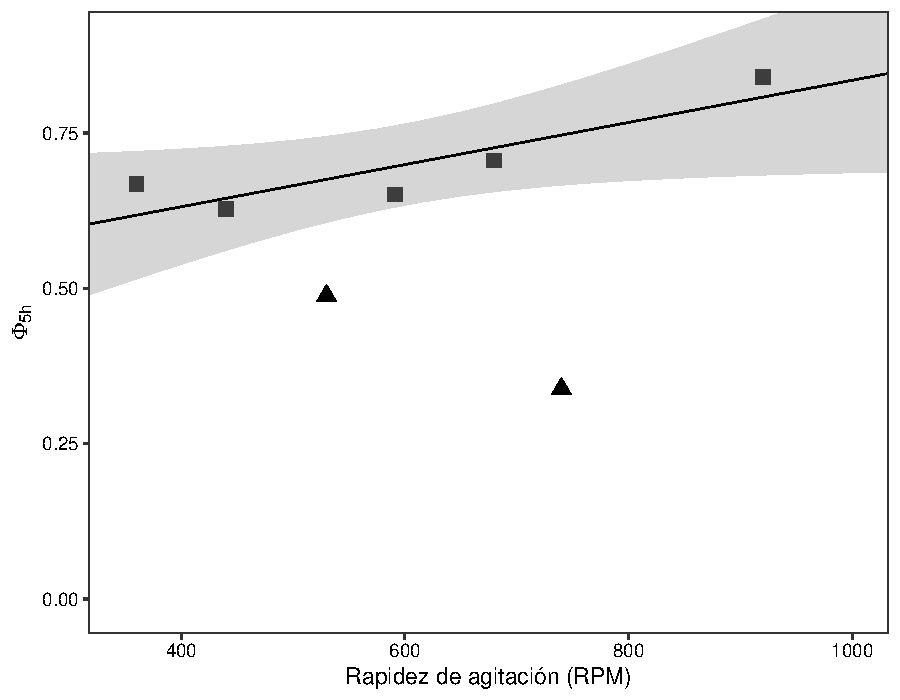
\includegraphics[height=0.375\textwidth, trim = {1.35cm 0 0 0},   clip]{chap5/figures/RPM_1.pdf}}
               \put(5, 160){\large b)}
               \end{picture}}\\
    \caption[Efecto de las condiciones hidrodinámicas en el proceso de transporte.]{Efecto de las condiciones hidrodinámicas en el proceso de transporte: (a) Perfiles de transporte de litio a distintos valores de rapidez de agitación (\protect\squareblck\ 360, \protect\circleblck\ 440, \protect\triangleupblck\ 530, \protect\circlewht\ 591, \protect\squarewht\ 680, \protect\squarerttdwht\ 740 y \protect\triangleupwht\ 920 RPM) y (b) fracción transportada de litio a las cinco horas en función de la rapidez de agitación (\protect\triangleupblck\ datos excluídos en la regresión). La zona sombreada corresponde al intervalo de confianza de la regresión a un nivel de confianza del 95\%.}
    \label{fig:RPM1}
\end{figure}

No parece haber una correlación fuerte entre la rapidez de agitación y la eficiencia del proceso de transporte. Si se excluyen los valores obtenidos a 530 y 740 RPM la relación es estadísticamente significativa (valor p de la prueba F sobre el modelo de regresión: 0.048), pero la distribución de los residuales de la regresión no es aleatoria, lo que indica que el modelo no describe adecuadamente el comportamiento de los datos. 

En principio, se esperaría que un aumento en la rapidez de agitación tenga un efecto positivo en la rapidez a la que el ion litio es transportado a través de la membrana hasta alcanzar un valor límite a partir del cual la rapidez de agitación no influye en la cinética del proceso. Esto se supone considerando que una rapidez de giro mayor en la propela hace más eficiente la homogeneización del seno de la disolución disminuyendo el grosor de la capa de difusión que deben atravesar las especies para llegar a la interfaz disolución-membrana. A partir de un valor límite, el grosor de la capa de difusión no puede disminuir más y la cinética del proceso queda controlada únicamente por la rapidez de la reacción interfacial de complejación y la velocidad a la que el aducto que se forma es transportado al otro lado de la membrana. 

En el gráfico de la Figura \ref{fig:RPM1}(b) no se observa ninguna región estacionaria. El transporte ineficiente que se obtuvo a 740 RPM puede justificarse por la formación de un régimen turbulento que es difícil de controlar a altos valores de $\Theta$. El efecto de la agitación parece no tener gran importancia en el intervalo de valores de rapidez de agitación entre 400 y 680 RPM.

Se evaluó la reproducibilidad del proceso a agitando las semiceldas a valores entre 510 y 585 \ac{RPM}. Los perfiles de transporte de litio y los factores de separación respecto al sodio se muestran en la Figura \ref{fig:RPM2}. Se bloqueó la variable \textit{Celda de transporte} (Celda 1 y 2) y se aleatorizó la variable \textit{rapidez de agitación} ($\Theta$).

\begin{figure}[H]
    \centering
    \subbottom{\begin{picture}(240,167)
               \put(0, 0){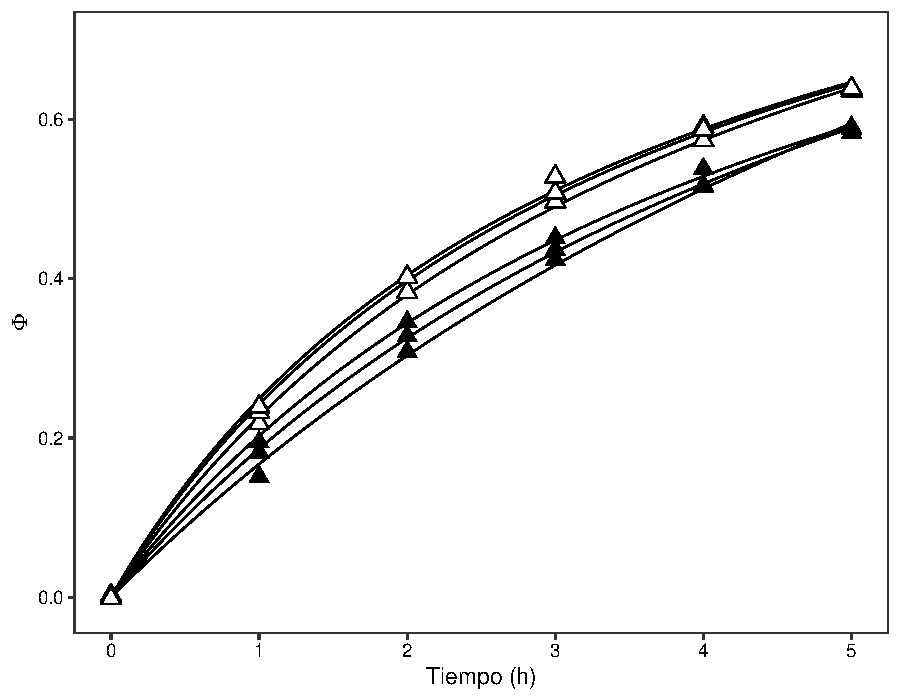
\includegraphics[height=0.37\textwidth, trim = {0cm 0 0 0},   clip]{chap5/figures/Theta2_profiles.pdf}}
               \put(0, 161){\large a)}
               \end{picture}}%
    \subbottom{\begin{picture}(250,167)
               \put(0, 0){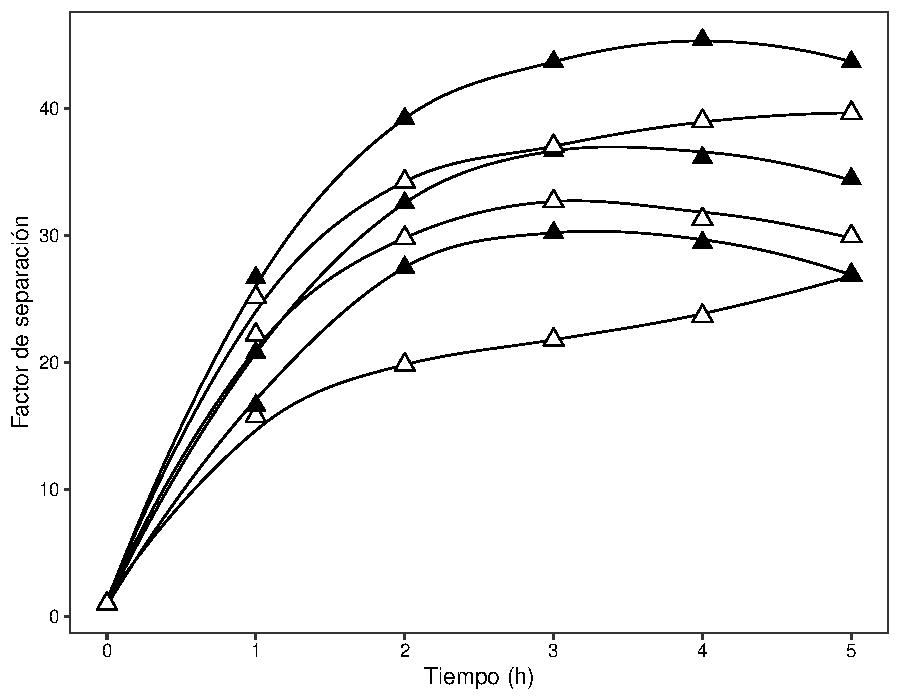
\includegraphics[height=0.37\textwidth, trim = {0cm 0 0 0},   clip]{chap5/figures/SepFactor_Thetha2.pdf}}
               \put(0, 161){\large b)}
               \end{picture}}\\
    \caption[Reproducibilidad del proceso de transporte.]{Reproducibilidad del proceso de transporte: (a) Perfiles de transporte de litio a la disolución de alimentación  y (b) factor de separación en función del tiempo para los distintos sistemas en la Celda 1 (\protect\triangleupblck) y en la Celda 2 (\protect\triangleupwht).}
    \label{fig:RPM2}
\end{figure}
\clearpage
Hay diferencias estadísticamente significativas\footnote{A un valor de confianza del 95\%. Valor p de la prueba t de igualdad de medias sobre la fracción transportada de litio a las cinco horas: 0.002} entre los transportes realizados en la celda 1 o en la celda 2. Los factores de separación presentan una gran variabilidad que parece ser independiente de la celda en la que se lleva a cabo el transporte y de la rapidez con la que se agiten las semiceldas. La desviación estándar relativa de la fracción transportada de litio a la disolución de alimentación está entre 15\% y 5\% para tiempos de una y cinco horas, respectivamente. La desviación estándar relativa del factor de separación es de 20\% y se mantiene relativamente contante en el tiempo. Considerando en conjunto los transportes realizados en cada celda, la desviación estándar relativa de los parámetros $\alpha$ y $\beta$ es de alrededor del 5\% (con la excepción del parámetro $\beta$ para los transportes en la celda 1 que es del 20\%). 

Se decidió trabajar únicamente con la celda 2 para los demás experimentos de transporte porque la celda 1 se descontrolaba con regularidad, produciendo derrames y haciendo más desgastantes los experimentos. Adicionalmente, los transportes de ion litio realizados en la celda 2 fueron más eficientes. 

%\subsubsection{Tercer diseño factorial fraccionado}
%En un intento por mejorar la eficiencia y la selectividad del sistema modificando algunas variables categóricas, se desarrollo un tercer diseño factorial fraccionado en el que se evaluaron tres parámetros: disolvente empleado en la preparación de la membrana (\textbf{X1}), morfología de la caja de petri usada como molde (\textbf{X2}). y disolución expuesta a la cara rugosa de la membrana (\textbf{X3}). La matriz de diseño se muestra en la Tabla \ref{tab:frf2matrix3}. Las membranas y las disoluciones de alimentación y de recuperación utilizadas son de la misma composición que las utilizadas en la Sección \ref{sec:hydroexpe}


%\subsubsection{Reproducibilidad del sistema}
%Previa a la optimización final del sistema es necesario conocer la reproducibilidad del mismo para establecer que diferencias en los resultados pueden considerarse importantes estadísticamente. Idealmente este proceso tuvo que haberse hecho antes del estudio del sistema haciendo uso de los experimentos factoriales fraccionados descritos en secciones anteriores.

\subsection{Optimización simplex}\index{Diseño de experimentos!algoritmo símplex}
Para optimizar el sistema se consideraron las variables masa de mezcla de extractantes (\textbf{X1}), relación molar LIX-54-100/Cyanex~923 (\textbf{X2}), concentración inicial de hidróxido de amonio en la disolución de alimentación (\textbf{X3}) y concentración inicial de ácido clorhídrico en la disolución de recuperación (\textbf{X4}). La masa de \ac{CTA} en las membranas se mantuvo constante en 30~mg. El objetivo de la optimización fue aumentar la velocidad del proceso de transporte, por lo que se consideró la maximización del parámetro promediado $\beta$ de los perfiles de transporte modelados usando la Ecuación \ref{eq:NLSCRIS} propuesta en el Capítulo \ref{sec:NLS}.

Para monitorear el factor de separación, se dispuso cloruro de sodio en la disolución de alimentación a una concentración tal que la relación molar \ce{Li+}/\ce{Na+} fuese de 1:10. El punto inicial del simplex y el tamaño de paso configurado se muestran en la Tabla \ref{tab:smplx2.1}. En la misma tabla se incluyen las coordenadas del simplex inicial generado junto con la respuesta obtenida para cada punto.

\begin{table}[H]
    \centering\footnotesize
    \begin{tabular}{@{}l c c c c c@{}}\toprule
         \textbf{ID}&\textbf{X1} (mg)&\textbf{X2}&\textbf{X3} (mol~kg\mnn)&\textbf{X4} (mol~kg\mnn)&$\overline{\beta}$\\\midrule
        \textit{Punto inicial}  & 70& 2.00& 0.010& 0.07&-\\
        \textit{Tamaño de paso} & 20 & 1.00& 0.010& -0.06&-\\\midrule
        \textbf{K.1} \textit{(vértice 1)}& \textbf{70.0}& \textbf{2.00}& \textbf{0.010}& \textbf{0.07}& \textbf{0.487}\\
        K.2&  50.0& 2.75& 0.010& 0.07& 0.397\\
        K.3&  50.0& 1.75& 0.016& 0.07& 0.254\\
        K.4&  50.0& 1.75& 0.007& 0.04& 0.268\\
        K.5&  50.0& 2.75& 0.007& 0.04& 0.345\\\bottomrule
    \end{tabular}
    \caption{Configuración del simplex inicial.}
    \label{tab:smplx2.1}
\end{table}

El proceso de optimización se completó con los puntos que se muestran en la Tabla \ref{tab:smplx2.2}. Los perfiles de transporte correspondientes al primer vértice (punto inicial de la optimización) y al vértice con la mejor respuesta (PIM K.9) se muestran en la Figura \ref{fig:simplex2.profiles}.
\begin{table}[H]
    \centering\footnotesize
    \begin{tabular}{@{}l l c c c c c@{}}\toprule
         \textbf{ID}&\textbf{Movimiento}&\textbf{X1} (mg)&\textbf{X2}&\textbf{X3} (mol~kg\mnn)&\textbf{X4} (mol~kg\mnn)&$\overline{\beta}$\\\midrule
         K.6&R&  60.0 & 2.88& 0.000& 0.04& 0.000\\
         K.7&Cw&  52.5& 2.03& 0.012& 0.06& 0.434\\
         K.8&R&  61.2& 3.02& 0.013& 0.08& 0.424\\
         \textbf{K.9}&\textbf{R}&  \textbf{66.8}& \textbf{2.15}& \textbf{0.016}& \textbf{0.10}& \textbf{0.554}\\
        K.10& E& 75.3& 1.85& 0.020& 0.13& 0.343\\
        K.11& R& 75.3& 1.85& 0.016& 0.09& 0.388\\
        K.12& Cw&56.3& 2.52& 0.011& 0.07& - \\\bottomrule
    \end{tabular}
    \caption{Vértices generados en el proceso de optimización.}
    \label{tab:smplx2.2}
\end{table}

\begin{figure}[H]
    \centering
    \subbottom{\begin{picture}(245,178)
               \put(0, 0){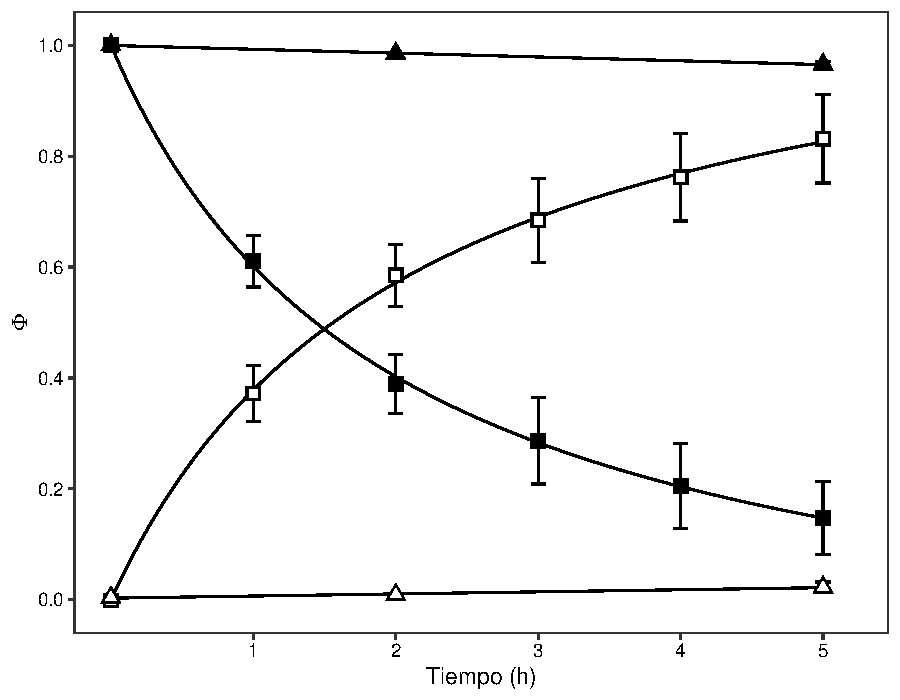
\includegraphics[height=0.388\textwidth]{chap5/figures/K1_pro.pdf}}
               \put(218, 167.5){\large a)}
               \end{picture}}%
    \subbottom{\begin{picture}(230,178)
               \put(0, 0){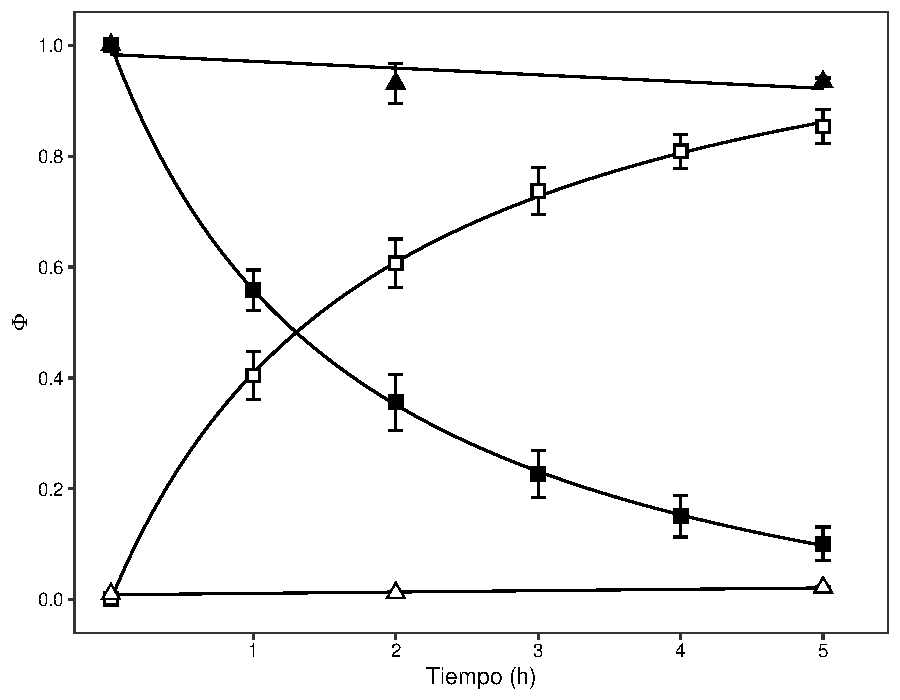
\includegraphics[height=0.388\textwidth, trim = {1.19cm 0 0 0},   clip]{chap5/figures/K9_pro.pdf}}
               \put(199, 167.5){\large b)}
               \end{picture}}
    \caption[Perfiles de transporte de litio del sistema bajo optimización.]{Perfiles de transporte de litio del punto inicial del simplex (a) y del vértice con la mejor respuesta considerado como el punto óptimo (b). Litio en la fase de alimentación (\protect\squareblck), litio en la fase de recuperación (\protect\squarewht), sodio en la fase de alimentación (\protect\triangleupblck) y sodio en la fase de recuperación (\protect\triangleupwht).}
    \label{fig:simplex2.profiles}
\end{figure}
De un total de 11 experimentos realizados, solo uno de los vértices obtuvo una respuesta mejor que la obtenida en el punto inicial del simplex. La optimización debe detenerse bajo el supuesto de que probablemente el sistema se encuentra muy cerca del punto óptimo y en esta zona el algoritmo de optimización resulta de poca utilidad para encontrar mejores condiciones \citep{simplexbook}. Las condiciones propuestas en el noveno vértice dan lugar a un transporte ligeramente mejor que el que se obtiene con las condiciones de cualquier otro vértice. La respuesta del noveno vértice es significativamente mejor que la del primer vértice, pero la diferencia no es muy grande. La optimización no resultó en una mejora sustancial del proceso de trasporte tal y como se pretendía.

%Los datos de las Tablas \ref{tab:smplx2.1} y \ref{tab:smplx2.2} permiten establecer que el transporte se ve menos favorecido si la masa de la mezcla de extractantes en la membrana es muy pequeña,

Se llevó a cabo el transporte de litio bajo las condiciones optimizadas sin incluir sodio en la di\-so\-lu\-ción de alimentación. El perfil de transporte para litio se muestra en la Figura \ref{fig:optim10}(a). El coeficiente de permeabilidad de litio puede obtenerse de la pendiente de la recta del logaritmo base 10 de la fracción remanente de litio en la disolución de alimentación en función del tiempo (Sección \ref{sec:performanceparameters}). La gráfica se muestra en la  Figura \ref{fig:optim10}(b) y el valor obtenido es de (2.13$\pm$0.04)\e{-5}~m~s\mnn. Hay una muy buena relación lineal entre los puntos representados y esto sustenta los supuestos que se hacen para calcular el coeficiente de permeabilidad para litio usando este método.
\begin{figure}[H]
    \centering
    \subbottom{\begin{picture}(245,171)
               \put(0, 0){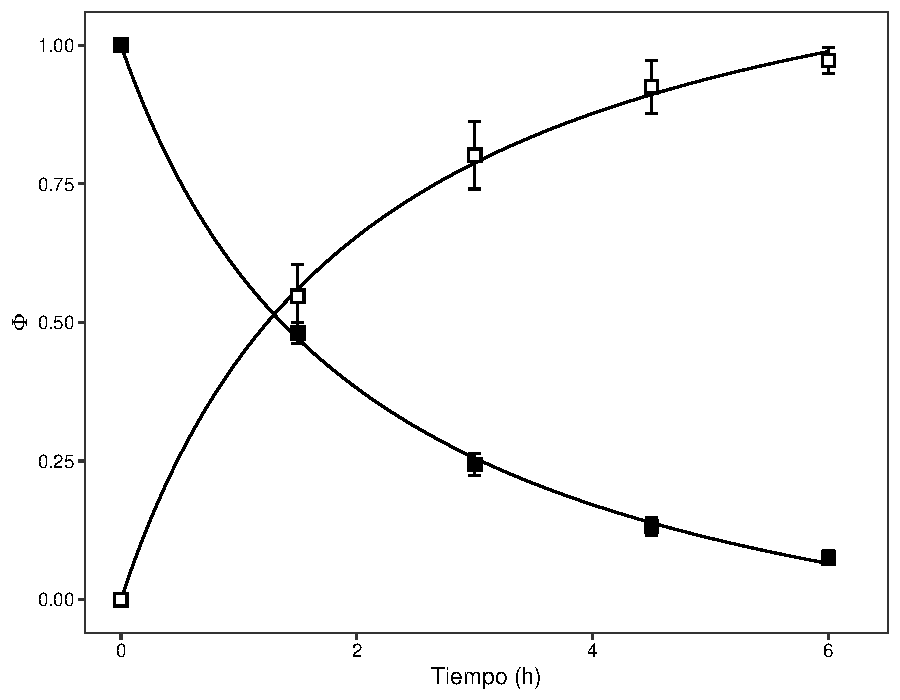
\includegraphics[height=0.383\textwidth]{chap5/figures/K10_pro.pdf}}
               \put(-1, 168){\large a)}
               \end{picture}}%
    \subbottom{\begin{picture}(230,178)
               \put(0, 0){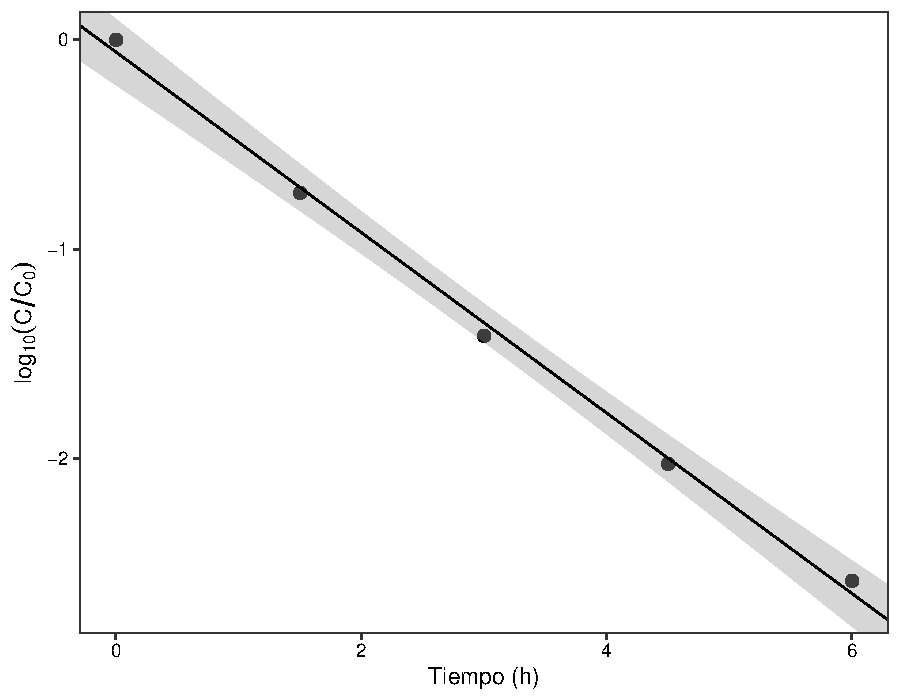
\includegraphics[height=0.383\textwidth, trim = {0 0 0 0},   clip]{chap5/figures/K10_perm.pdf}}
               \put(-1, 168){\large b)}
               \end{picture}}
    \caption[Perfil de transporte de litio del sistema optimizado.]{Perfil de transporte de litio bajo condiciones optimizadas (a) y gráfico del logaritmo base 10 de la fracción remanente de litio en la disolución de alimentación en función del tiempo para el calculo del coeficiente de permeabilidad (b). Litio en la fase de alimentación (\protect\squareblck), litio en la fase de recuperación (\protect\squarewht). La región sombreada corresponde a los intervalos de confianza de la regresión lineal a un nivel de confianza del 95\%. Coeficiente de permeabilidad: (2.13$\pm$0.04)\e{-5}~m~s\mnn}.
    \label{fig:optim10}
\end{figure}

\clearpage\section{Caracterización del sistema optimizado}
\subsection{Selectividad}\label{sec:selecresults}\index{PIM!Selectividad}
Los perfiles de transporte competitivo de ion litio contra sodio, potasio y magnesio en relaciones molares (\ce{Li+}/\ce{M^n+}) 1:1, 1:10 y 1:100 se muestran en la Figura \ref{fig:selectivity1}.

\begin{figure}[H]
    \centering
    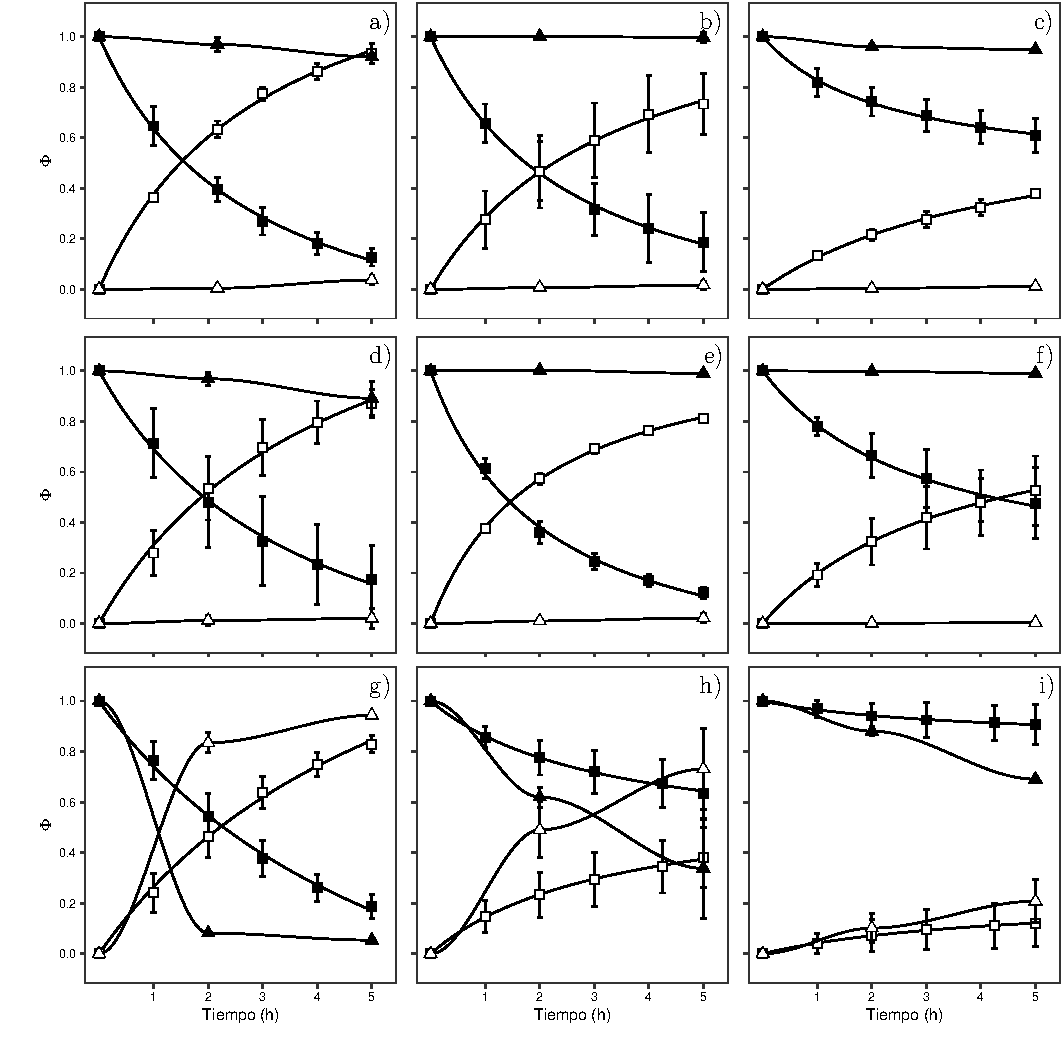
\includegraphics[width=\textwidth]{chap5/figures/thesis-selectividad.pdf}
    \caption[Perfiles de transporte competitivo de ion litio contra sodio, potasio y magnesio.]{Perfiles de transporte de ion litio en presencia de otros cationes interferentes a distintas relaciones molares: sodio 1:1 (a), sodio 1:10 (b), sodio 1:100 (c), potasio 1:1 (d), potasio 1:10 (e), potasio 1:100 (f), magnesio 1:1 (g),  magnesio 1:10 (h) y magnesio 1:100 (i). Ion litio en la fase de alimentación (\protect\squareblck), ion litio en la fase de recuperación (\protect\squarewht), catión interferente en la fase de alimentación (\protect\triangleupblck) y catión interferente en la fase de recuperación (\protect\triangleupwht).}
    \label{fig:selectivity1}
\end{figure}

\clearpage El sistema presenta buena selectividad frente a los cationes alcalinos sodio y potasio. La presencia de estos iones ocasiona una disminución considerable en la permeabilidad de la membrana frente a los iones litio. Este efecto es más marcado cuando las relaciones molares de sodio y de potasio respecto al ion litio son grandes. La fracción transportada de sodio y de potasio se mantiene baja y disminuye con el aumento en su concentración inicial en la disolución de alimentación. Esto se debe a que si la concentración de los iones en la disolución de alimentación es alta, una mayor cantidad neta debe ser transportada para observar un cambio apreciable en las fracciones de cada fase. En otros términos, esto implica que aunque la fracción transportada de sodio y potasio se mantiene baja, una cantidad apreciable de estos iones si es transportada ocupando sitios activos de la membrana y naturalmente, esto disminuye la eficiencia con la que el ion litio es extraído.

Un comportamiento muy diferente lo presenta el catión divalente magnesio que no es excluido por la PIM sino que es transportado incluso con mayor eficiencia que el ion litio. Esto se observa aún cuando su concentración molar es dos órdenes de magnitud mayor a la del ion litio. Varios autores \citep{Liu2020, Zhang2019} han atribuído la falta de selectividad hacia el magnesio por parte de varios de los sistemas destinados a la separación de ion litio al hecho de que los radios iónicos de estos elementos son muy similares: 69 y 72~pm para el ion litio y el magnesio, respectivamente \citep{Marcus1994}. Adicionalmente, el magnesio es un catión divalente y esto hace que en general sea más fuertemente solvatado que el ion litio, que es monovalente \citep{Israelachvili2011}. Se espera que el sistema también presente una pobre selectividad frente al catión calcio.  Los coeficientes de separación son función de la relación molar de cationes presente inicialmente \citep{Chen2018}. Como se observó en la Sección \ref{sec:reprod}, la reproducibilidad de estos valores no es buena.

%\begin{table}[H]
%    \centering
%    \subbottom[]{
%    \begin{tabular}{@{}l c c c @{}}\toprule
%        \multirow{2}{*}{\textbf{Especie}}&\multicolumn{3}{c}{\textbf{Rel. molar}}\\\cline{2-4}
%        & 1:1 & 1:10&1:100\\\midrule
%        Sodio    & 5.4 & 43 & \\
%        Potasio  & 8.0 & 36 & \\
%        Magnesio & >1 & >1& >1\\\bottomrule
%    \end{tabular}
%    }\hspace{5ex}
%    \subbottom[]{
%    \begin{tabular}{@{}l c c c @{}}\toprule
%        \multirow{2}{*}{\textbf{Especie}}&\multicolumn{3}{c}{\textbf{Rel. molar}}\\\cline{2-4}
%        & 1:1 & 1:10&1:100\\\midrule
%        Sodio    & 5.4 & 41 & 33\\
%        Potasio  & 8.0 & 36 & \\
%        Magnesio & >1 & >1& >1\\\bottomrule
%    \end{tabular}
%    }
%    \caption[Factores de separación de ion litio frente a sodio, potasio y magnesio a distintas relaciones molares]{Factores de separación máximos (a) y finales (b) para disoluciones de alimentación con ion litio y sodio, potasio o magnesio a distintas relaciones molares iniciales.}
%    \label{tab:sep-factorlinakmg}
%\end{table}

La aplicación del método a una matriz real (como agua de mar) requiere que el calcio y el magnesio sean retirados del medio antes de intentar la extracción de ion litio. La opción por excelencia es por precipitación selectiva aprovechando la baja solubilidad de distintas sales de estos elementos. Diversos protocolos se han propuesto para la precipitación de estos cationes usando por ejemplo metasilicato de sodio monohidratado \citep{Zhang2019}, ácido oxálico \citep{TRAN2015} o cloruro de potasio con monohidrógenofosfato de sodio en dos etapas \citep{Lai2020}. Las alternativas más comunes involucran precipitación en forma de hidróxidos alcalinizando el medio con hidróxido de sodio \citep{ALAMDARI2008} o hidróxido de amonio \citep{Harvianto2016}. 

La precipitación usando hidróxido de amonio es una idea seductora desde un punto de vista práctico porque no se adicionan cationes alcalinos al medio con lo que el ion litio no se vuelve más difícil de separar. Sin embargo, la precipitación cuantitativa de magnesio bajo estas condiciones no es posible debido a la formación de complejos amoniacales que solubilizan nuevamente al catión \citep{Yamagata2011}. Por otro lado, precipitar el magnesio es relativamente sencillo usando hidróxido de sodio, pero la precipitación cuantitativa de calcio se obtiene a un pH mayor a 13, con lo que la concentración de iones sodio en el medio debería ser aumentada considerablemente. 

\citet{AN2012b} encontraron que la mejor manera de eliminar cationes interferentes de salmueras del Salar de Uyuni (Bolivia) era por medio de una precipitación en dos pasos usando inicialmente carbonato de sodio y posteriormente oxalato de sodio. Este enfoque mitiga el aumento de especies indeseables en la disolución resultante. Con el fin de minimizar el aumento de iones sodio y de remover cuantitativamente los iones calcio y magnesio del agua de mar, se determinó experimentalmente que el magnesio y una fracción importante del calcio pueden retirarse con la adición de hidróxido de sodio a una concentración final de 0.15~mol~kg\mnn. Los iones calcio remanentes son retirados por completo en un paso posterior añadiendo monohidrógenofosfato de amonio a una concentración final de 0.005~mol~kg\mnn. La concentración promedio de iones sodio en agua de mar es de 0.47~mol~kg\mnn \citep{Dickson1994}. El hidróxido de sodio añadido representa un aumento de más del 30\% en la concentración de este catión, pero dado que en agua de mar la relación molar \ce{Na+}/\ce{Li+} es de alrededor de 18000, el panorama no empeora significativamente. Los detalles experimentales de este protocolo se describieron en la Sección \ref{sec:preci}.

\citet{Diaz2019} propusieron una alternativa muy limpia para remover los iones calcio y magnesio presentes en salmueras de ion litio usando electrólisis de membrana en una celda especial. La metodología propuesta permite obtener por separado hidróxido de magnesio e hidróxido de calcio usando hidróxidos provenientes, de la electrólisis reductiva del agua que los contiene. La semireacción que completa la celda electrolítica produce iones hidronio que podrían neutralizar el medio y resolubilizar los hidróxidos recientemente formados pero para evitar esto, el ánodo se encuentra en un compartimiento diferente, separado por una membrana intercambiadora de aniones que no permite su paso hacia el compartimiento donde se encuentra la salmuera bajo tratamiento. Este método no involucra la adición de reactivos precipitantes, sino que estos son generados \textit{in situ}. Los subproductos generados pueden tener valor comercial y la matriz no se hace más compleja (no aumenta la concentración de iones sodio) como consecuencia del proceso. 

\subsection{Capacidad de reuso}\label{sec:reuseres}\index{PIM!estabilidad}
Los perfiles de ion litio remanente en la disolución de alimentación en función del tiempo para los distintos ciclos de extracción de ion litio a partir de una disolución de alimentación ideal se muestran en la Figura \ref{fig:cycles}(a). La fracción transportada de ion litio hacia la disolución de alimentación tras seis horas de cada ciclo se resume en la Figura \ref{fig:cycles}(b).

La eficiencia de la membrana decae casi constantemente tras cada ciclo de reuso. Luego de 10 ciclos de transporte ha perdido cerca del 40\% de la capacidad inicial de la membrana y tiempos mayores pueden ser requeridos para extraer una fracción de ion litio similar a cuando se usa una membrana nueva. La inestabilidad de la membrana puede atribuirse a la alcalinidad de la di\-so\-lu\-ción de alimentación y a la suceptibilidad de las $\beta$-dicetonas (como el LIX-54-100) de lixiviarse desde la PIM bajo estas condiciones \citep{Sugiura1989}.

\begin{figure}[H]
    \centering
    \subbottom{\begin{picture}(242,170)
               \put(0, 0){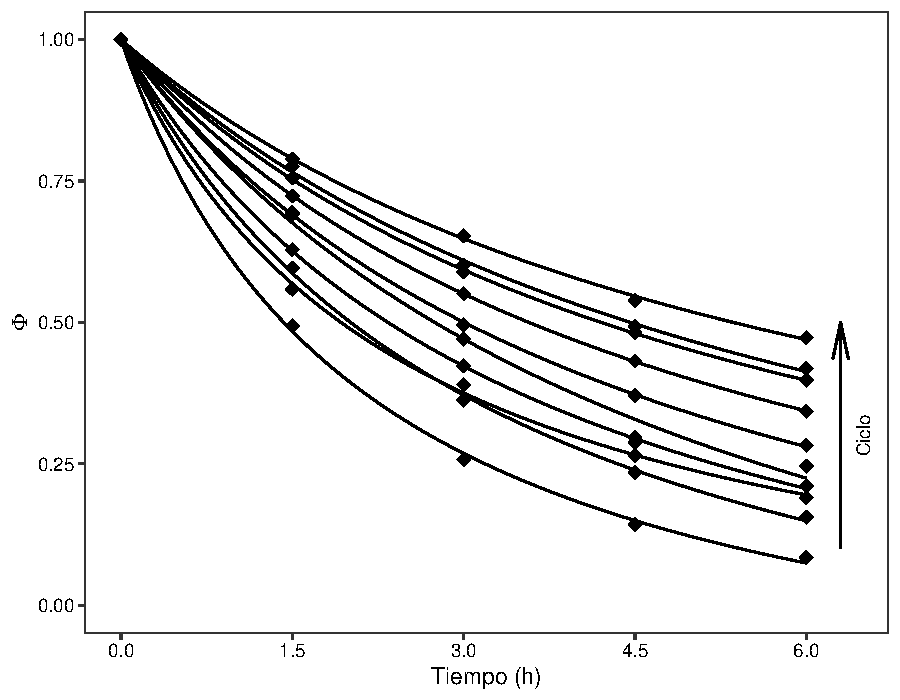
\includegraphics[height=0.388\textwidth]{chap5/figures/reuseprofiles.pdf}}
               \put(219, 168){\large a)}
               \end{picture}}%
    \subbottom{\begin{picture}(230,170)
               \put(0, 0){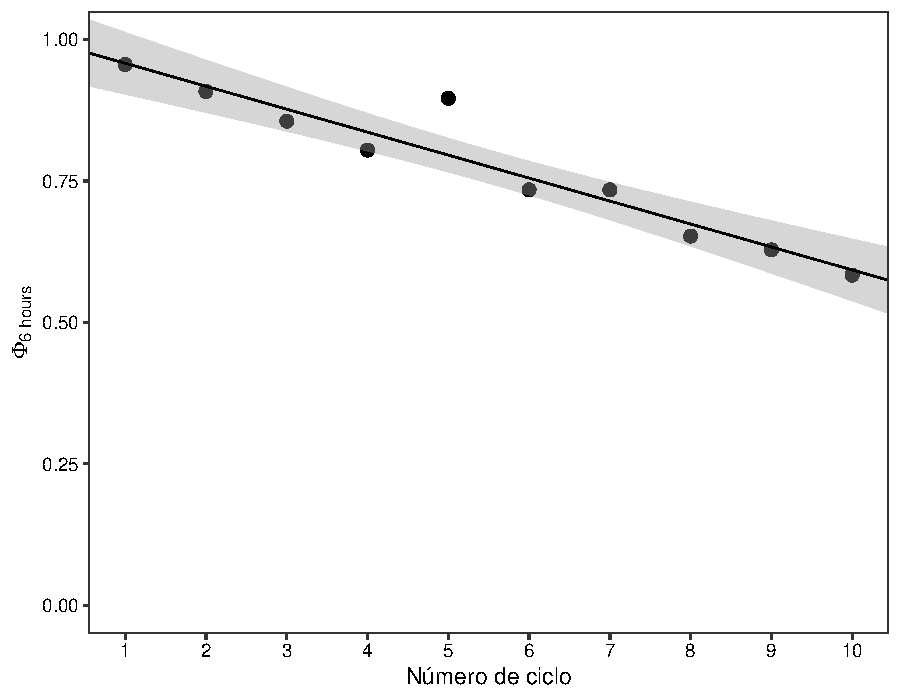
\includegraphics[height=0.388\textwidth, trim = {1.35cm 0 0 0},   clip]{chap5/figures/reusesummary.pdf}}
               \put(197, 168){\large b)}
               \end{picture}}\\
    \caption[Transporte de ion litio en varios ciclos reutilizando la membrana.]{Transporte de ion litio en varios ciclos reutilizando la membrana. (a) Perfiles de transporte desde la disolución de alimentación y (b) fracción transportada de ion litio hacia la disolución de recuperación tras seis horas en cada ciclo. La zona sombreada corresponde al intervalo de confianza de la regresión a un nivel de confianza del 95\%.}
    \label{fig:cycles}
\end{figure}

\subsection{Capacidad de concentración de ion litio}\label{sec:idealconc}
Con los resultados de secciones anteriores se conoció que el sistema es capaz de transportar ion litio en contra de su gradiente de concentración. Esto es posible si su transporte se acopla un contratransporte de iones hidronio. Tras la observación de que la membrana podía ser reutilizada para transportar ion litio se llevó a cabo un experimento similar en el que no se renovó la disolución de recuperación al final de cada ciclo con el propósito de obtener ion litio a una concentración mayor que la disponible inicialmente en la disolución de alimentación. El proceso de transporte se llevó a cabo bajo estas condiciones durante cinco ciclos y el perfil de transporte de ion litio se muestra en la Figura \ref{fig:liconc1}. 

El factor de concentración es de 3.2 luego de cinco ciclos de transporte de ion litio. Esto es equivalente a una eficiencia global de 64\%. Se observa que con cada cambio de la disolución de alimentación disminuye la eficiencia del proceso, como ya se había observado en la Sección \ref{sec:reuseres}. La concentración de ion litio es factible usando la metodología propuesta.

\begin{figure}[H]
    \centering
    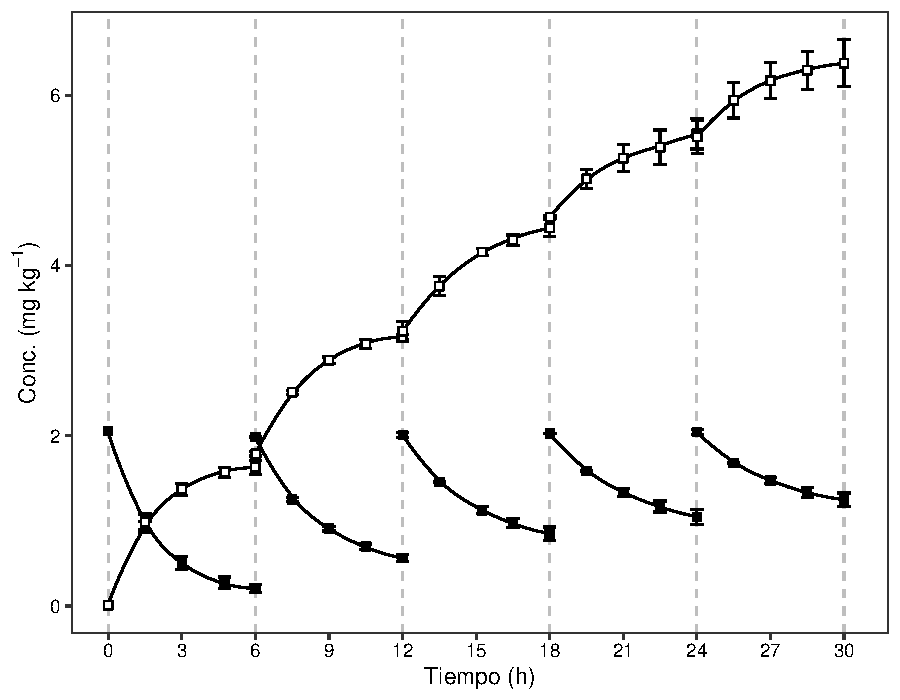
\includegraphics[width = 0.6\textwidth]{chap5/figures/liconc_0.pdf}
    \caption[Concentración de ion litio a partir de una disolución de alimentación ideal.]{Perfil de concentración de ion litio a partir de una disolución de alimentación ideal. Las líneas descontinuas verticales corresponden al inicio o al final de cada ciclo. (\protect\squareblck) ion litio en las disoluciones de alimentación y (\protect\squarewht) ion litio en la disolución de recuperación.}
    \label{fig:liconc1}
\end{figure}


\section{Agua de mar}\label{sec:resultsSSS}\index{Agua de mar}
Como ya se comentó en la Sección \ref{sec:selecresults}, el sistema no es selectivo frente al magnesio y probablemente tampoco lo sea frente al calcio. Estos cationes deben ser retirados del agua de mar antes de intentar extraer el ion litio. La relación molar \ce{Mg^2+}/\ce{Li+} y \ce{Ca^2+}/\ce{Li+} en agua de mar es de 2030:1 y 400:1, respectivamente \citep{Dickson1994}. La concentración final remanente de iones hidroxilo luego del proceso de precipitación por pasos usando hidróxido de sodio y monohidrógenofosfato de amonio se encuentra entre 0.03 y 0.04~mol~kg\mnn. La alcalinidad resultante del medio lo hace adecuado para su uso directo como disolución de alimentación sin la necesidad de añadir reactivos adicionales. 

El perfil de transporte de ion litio, sodio y potasio usando agua de mar sintética simplificada luego de la remoción de iones calcio y magnesio se muestra en la Figura \ref{fig:SSS1}(a). Los factores de separación de ion litio contra sodio y potasio se presentan en la  Figura \ref{fig:SSS1}(b).

El ion litio parece ser transportado en su totalidad hacia la disolución de recuperación tras 4.5 horas de iniciado el proceso. La concentración a la que se encuentra el ion litio en esta matriz es de 0.18~mg~kg\mnn, cerca de diez veces menor a la que contenía la disolución de alimentación con la que el proceso fue optimizado. Para un volumen constante, una menor concentración de ion litio en la disolución de alimentación hace que los cambios de esta magnitud en esta disolución como consecuencia del proceso de transporte, representen una proporción mayor de la especie presente al comienzo del experimento. Debido a esto, la depleción de iones litio de la disolución ocurre en un intervalo de tiempo más corto.  Por otro lado, debe considerarse que la concentración de iones sodio y potasio en el medio es muy alta. Aunque el sistema es muy selectivo frente a estos cationes, se demostró en la Figura \ref{fig:selectivity1} que cuando estas sustancias están a altas concentraciones, su cotransporte afecta de manera importante el transporte de ion litio.

\begin{figure}[H]
  \centering
    \subbottom{\begin{picture}(240,167)
               \put(0, 0){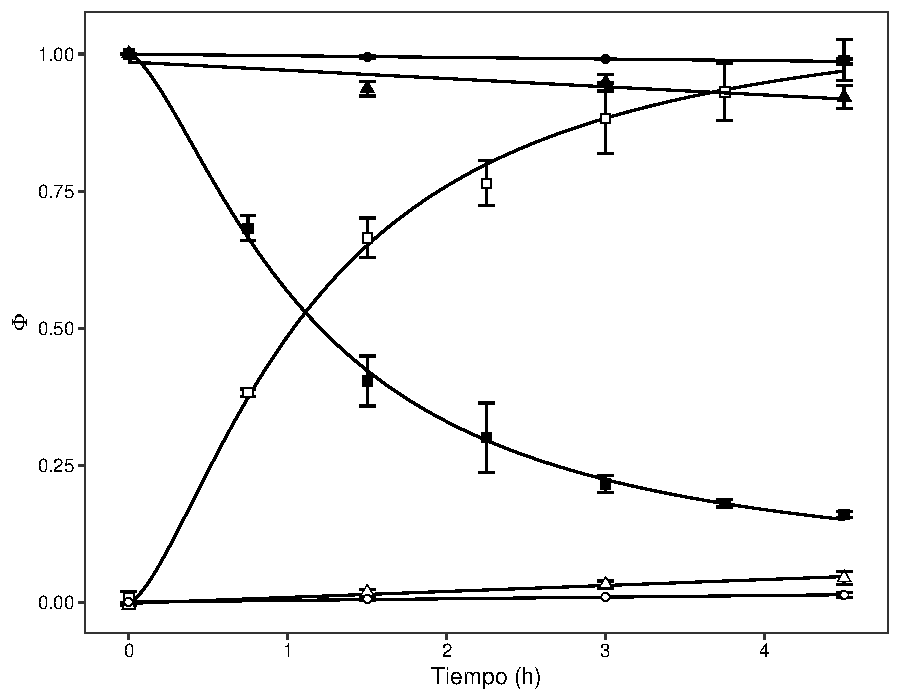
\includegraphics[height=0.37\textwidth, trim = {0cm 0 0 0},   clip]{chap5/figures/sssprof.pdf}}
               \put(-1, 161){\large a)}
               \end{picture}}%
    \subbottom{\begin{picture}(250,167)
               \put(0, 0){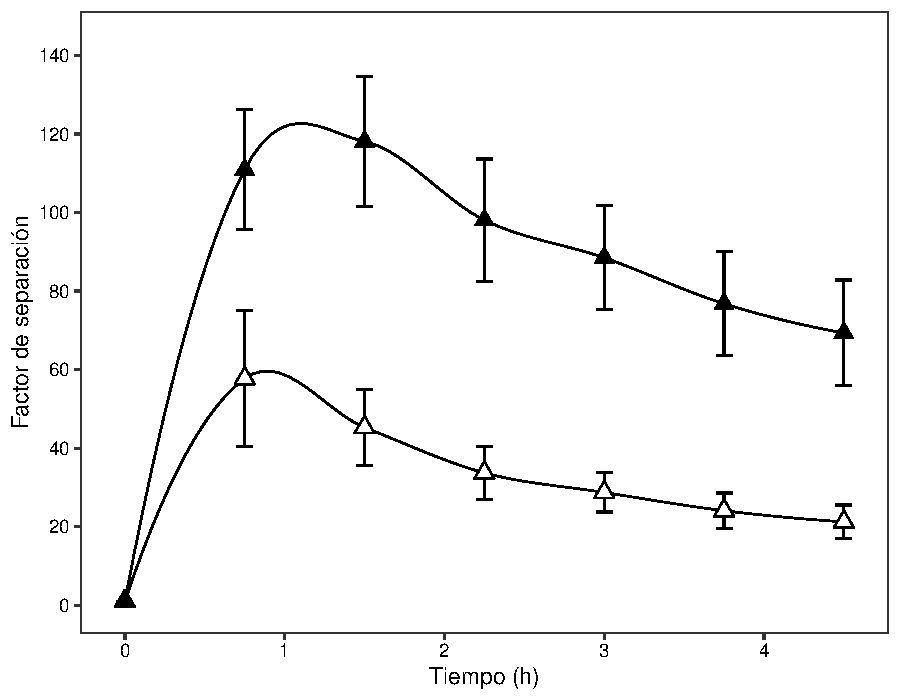
\includegraphics[height=0.37\textwidth, trim = {0cm 0 0 0},   clip]{chap5/figures/sssSep.pdf}}
               \put(-1, 161){\large b)}
               \end{picture}}\\
    \caption[Perfil de transporte y factores de separación usando agua de mar sintética simplificada.]{(a) Perfil de transporte usando agua de mar sintética simplificada: ion litio en la fase de alimentación (\protect\squareblck), ion litio en la fase de recuperación (\protect\squarewht), sodio en la fase de alimentación (\protect\triangleupblck), sodio en la fase de recuperación (\protect\triangleupwht), potasio en la fase de alimentación (\protect\circleblck) y potasio en la fase de recuperación (\protect\circlewht).  (b) factores de separación en función del tiempo: (\protect\triangleupblck) \ce{Li+}/\ce{K+} y (\protect\triangleupwht) \ce{Li+}/\ce{Na+}.}
  \label{fig:SSS1}
\end{figure}


En la Figura \ref{fig:SSS1}(a), la disolución de alimentación parece quedar hacia el final del proceso con un remanente del 15\% del ion litio presente inicialmente. Esto no concuerda con el perfil de transporte de ion litio hacia la disolución de recuperación en  donde aparentemente todo el ion litio es transportado al otro lado de la PIM. Esta posible inconsistencia en el balance de materia del sistema puede justificarse por un efecto matriz de naturaleza traslacional para la cuantificación de ion litio en la matriz de agua de mar. La cuantificación de ion litio se hizo por adición estándar de un punto (ver Anexo \ref{sec:quantification}) y esto mejoró significativamente el balance de materia para ion litio en las disoluciones corrigiendo los efectos matriz rotacionales debidos a los componentes presentes en el agua de mar. Sin embargo, la cuantificación por adición estándar de un solo punto es incapaz de corregir efectos matriz traslacionales \citep{Ellison2008}. Estos efectos matriz difíciles de corregir tienen un efecto más marcado a bajas concentraciones de ion litio. Es probable que en nuestro caso particular, el sesgo introducido cuando la concentración de ion litio es casi nula corresponda a una fracción de 0.15.

Los factores de separación máximos alcanzados frente a sodio y potasio son 118$\pm$16 y 57$\pm$17, respectivamente. Los factores de separación finales frente a sodio y potasio son 69$\pm$13 y 21$\pm$4, respectivamente. El sistema es capaz de selectivamente extraer ion litio de agua de mar.

\subsection{Muestras reales}
\subsubsection{Caracterización}
La concentración de iones litio, sodio, potasio, magnesio y calcio determinadas en las muestras de agua de mar natural recolectadas se muestra en la Tabla \ref{tab:swChar}
\begin{table}[H]
    \centering\footnotesize
    \begin{tabular}{@{}lccccc@{}}\toprule
        \multirow{2}{*}{\textbf{Procedencia}}&[\ce{Li^+}]&[\ce{Na^+}]&[\ce{K^+}]&[\ce{Mg^2+}]&[\ce{Ca^2+}]\\ 
        &(mg~kg\mnn)&(mg~kg\mnn)&(mg~kg\mnn)&(mg~kg\mnn)&(mg~kg\mnn)\\\midrule
        St.\ George Island, Estados Unidos &0.22$\pm$0.03 &~~9870$\pm$110 &359$\pm$22& 1173$\pm$32& 369$\pm$4\\[0.5ex]
        Santa Marta, Colombia &0.23$\pm$0.01 &10732$\pm$134 &401$\pm$10& 1278$\pm$33& 393$\pm$1\\[0.5ex]
        Referencia \citep{Trujillo2016} &0.18&10784&399&1284&415\\\bottomrule
    \end{tabular}
    \caption{Concentración de cationes en las muestras de agua de mar natural.}
    \label{tab:swChar}
\end{table}
La salinidad superficial del agua de mar tiende a ser mayor en inmediaciones a los Trópicos de Cáncer y Capricornio que en la Línea Ecuatorial \citep{Trujillo2016}. Esto se debe a una combinación de factores ambientales que favorecen la evaporación de agua en la zona de los trópicos aumentando la concentración de sales en el agua. La evaporación masiva de agua en la zona Ecuatorial también es un factor importante pero a diferencia de la zona de los Trópicos, la precipitación constante de agua fresca aminora el impacto que esto genera.

Contrario a lo descrito en el párrafo anterior, el agua proveniente de St.\ George Island, Estados Unidos, presenta una concentración menor de cationes respecto al agua muestreada en Santa Marta, Colombia. Esto puede atribuírse a que la isla se encuentra en la Bahía de Apalachicola, donde desemboca el agua dulce del Río Apalachicola. Este es el río más grande del Estado de Florida. El agua del río diluye levemente el agua salada que rodea la isla donde fue tomada la muestra de agua. Por otro lado, la única fuente de `agua dulce' cercana al punto de muestreo en Colombia es el Río Manzanares\footnote{El Río Manzanares sufre de un terrible daño ambiental por descarga de aguas residuales y de varias toneladas de basura al año \citep{Iguaran2019}. Lamentablemente, hace muchos años que sus aguas dejaron de ser \textit{dulces}.}. El caudal del Río Manzanares es pequeño y la Bahía de Santa Marta donde desemboca se encuentra más abierta al mar con lo que la dilución de las sales disueltas en el agua marina es mucho menor.

\subsubsection{Extracción y concentración de ion litio}

Las muestras procedentes de las dos locaciones fueron mezcladas y se removieron los iones calcio y magnesio por precipitación/centrifugación. Se llevaron a cabo cuatro ciclos de extracción de ion litio renovando la disolución de agua de mar en el compartimiento de alimentación. Cada ciclo tuvo una duración de 4.5 horas. 

La concentración de ion litio no es factible usando el sistema propuesto si no se reajusta la concentración de iones hidronio en la disolución de recuperación al final de cada ciclo de transporte. La acidez de la disolución de recuperación disminuye gradualmente y al volverse alcalina esta disolución, el transporte de ion litio no solo se detiene, sino que incluso es transportado de regreso hacia la disolución de alimentación como se muestra a partir del tercer ciclo en la Figura \ref{fig:FAIL}. 

\begin{figure}[H]
    \centering
    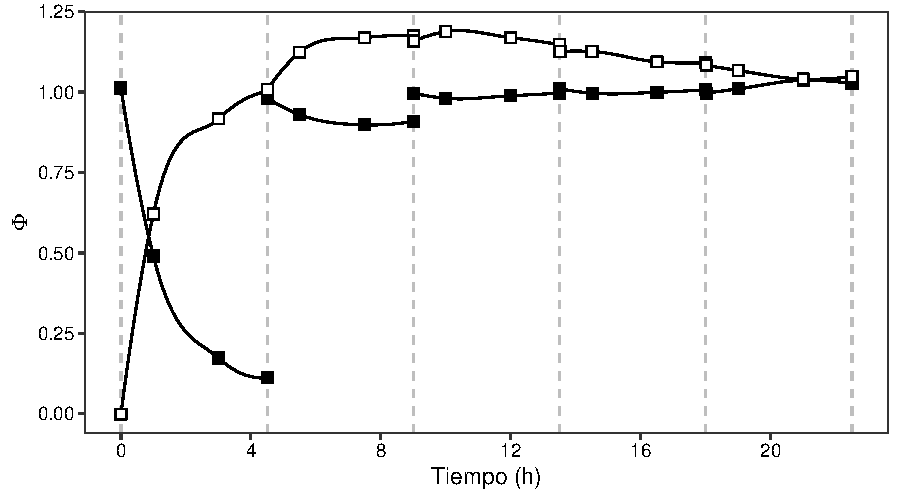
\includegraphics[width=0.65\textwidth, trim = {0cm 0 0 0},   clip]{chap5/figures/LiConcAS-FAIL.pdf}
    \caption[Concentración de ion litio sin reajustar la acidez en la fase de recuperación.]{Perfil de transporte de ion litio cuando se intenta concentrar a partir de agua de mar natural sin reajustar la concentración de iones hidronio en la disolución de recuperación al final de cada ciclo. (\protect\squareblck) ion litio en las disoluciones de alimentación y (\protect\squarewht) ion litio en la disolución de recuperación.}
    \label{fig:FAIL}
\end{figure}

La concentración de iones hidronio en la disolución de recuperación debe ser reajustada al valor original de 0.10~mol~kg\mnn\ al final de cada ciclo de extracción. La disminución en la concentración de iones hidronio en la fase de recuperación no fue importante cuando el ion litio se concentró a partir de una disolución de alimentación ideal. Cuando se usa agua de mar, el flujo de sodio y potasio hacia la disolución de recuperación es significativo a pesar de la buena selectividad del sistema. El flujo de cationes hacia la fase de recuperación conlleva un agotamiento de iones hidronio desde la misma. Si el flujo de cationes es significativo como en este caso, la disolución de recuperación puede volverse alcalina, y al desaparecer el gradiente de iones hidronio el transporte activo de iones litio se detiene. 

Se hizo un nuevo experimento reajustando la concentración de iones hidronio en la fase de recuperación al comienzo de cada ciclo. La concentración de iones litio, sodio, y potasio fue monitoreada en ambas disoluciones durante todo el proceso y los perfiles de transporte obtenidos se muestran en la Figura \ref{fig:liconcSW}. Puede observarse que reajustar la concentración de iones hidronio al final de cada ciclo parece ser suficiente para lograr la concentración de ion litio. Otra alternativa pudo haber sido mantener constante la acidez de esta disolución, por medio de la adición de sustancias amortiguadoras de pH. Esta opción no fue evaluada porque se deseó mantener la matriz de la disolución de alimentación tan simple como fuese posible.

\begin{figure}[htbp]
    \centering
    \subbottom{\begin{picture}(330,145)
               \put(0, 0){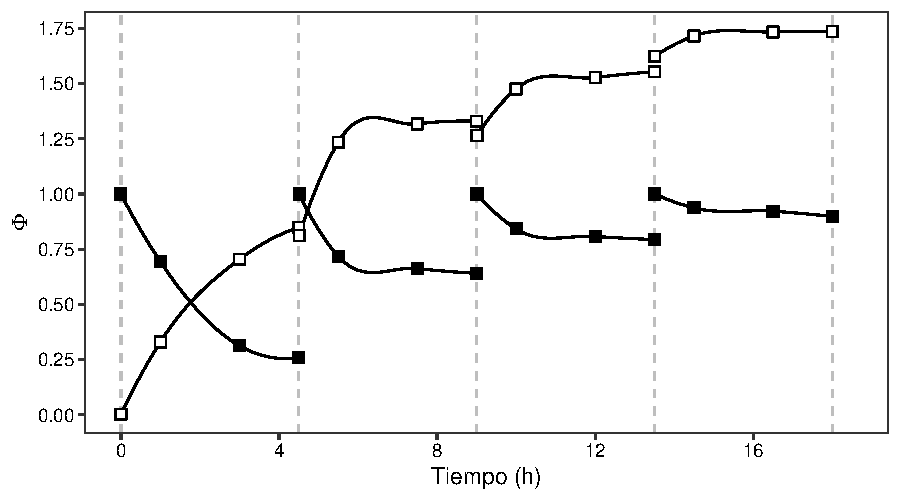
\includegraphics[width=0.65\textwidth, trim = {0cm 0.96cm 0 0},   clip]{chap5/figures/LiConcAS.pdf}}
               \put(-1, 137){\large a)}
               \end{picture}}\\
    \subbottom{\begin{picture}(330,145)
               \put(0, 0){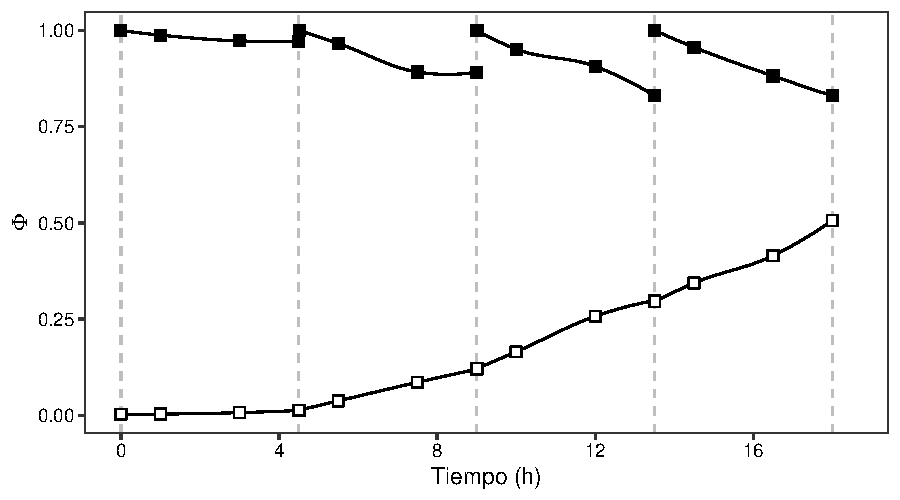
\includegraphics[width=0.65\textwidth, trim = {0cm 0.96cm 0 0},   clip]{chap5/figures/NaConcAS.pdf}}
               \put(-1, 137){\large b)}
               \end{picture}}\\
    \subbottom{\begin{picture}(330,165)
               \put(0, 0){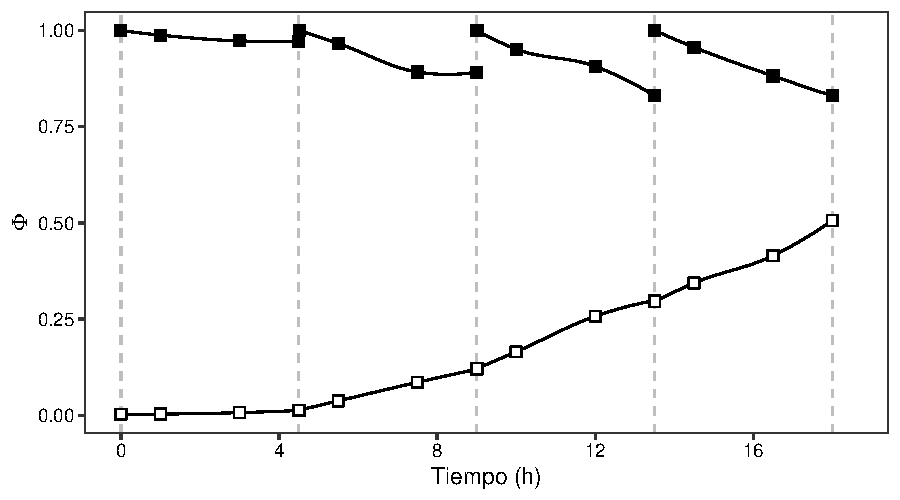
\includegraphics[width=0.65\textwidth, trim = {0cm 0 0 0},   clip]{chap5/figures/KConcAS.pdf}}
               \put(-1, 155){\large c)}
               \end{picture}}
    \caption[Concentración selectiva de ion litio a partir de agua de mar natural.]{Perfil de transporte de ion litio (a), ion sodio (b), e ion potasio (c) a partir de agua de mar natural sin calcio ni magnesio. Las líneas descontinuas verticales corresponden al inicio o al final de cada ciclo. (\protect\squareblck) especie en las disoluciones de alimentación y (\protect\squarewht) especie en la disolución de recuperación.}
    \label{fig:liconcSW}
\end{figure}

La capacidad de la membrana para extraer ion litio se ve deteriorada tras cada ciclo. El perfil de transporte para la concentración de ion litio usando agua de mar (Figura \ref{fig:liconcSW}(a)) difiere significativamente del obtenido cuando se usa una disolución de alimentación sin interferentes (Figura \ref{fig:liconc1}). Al usar una disolución de alimentación ideal, las pérdidas en la eficiencia del transporte disminuyen sutilmente tras cada ciclo y la membrana opera casi al 50\% de su capacidad en el quinto ciclo de concentración. Cuando se usa agua de mar, la eficiencia del sistema en el segundo ciclo es la mitad de la obtenida en el primer ciclo. En el cuarto ciclo la cantidad de ion litio extraído es solo el 13\% del que se extrae en el primer ciclo.

Un comportamiento muy diferente se observa para los cationes interferentes sodio y potasio. La fracción extraída de estos iones al final de cada ciclo es cada vez mayor. Excluyendo los cationes divalentes, la selectividad del sistema es \ce{Li+} $\gg$ \ce{Na+} > \ce{K+} (ver Sección \ref{sec:selecresults}). A partir del segundo ciclo, el orden entre sodio y potasio se invierte y el sistema empieza a extraer potasio con mayor eficiencia que con la que extrae sodio. En el cuarto ciclo la fracción de potasio que es transportada desde la disolución de alimentación es mayor a la de ion litio en casi un 10\%. Esto se presenta a pesar de que el potasio se encuentra en un exceso molar respecto al ion litio de casi 400:1. La selectividad del sistema para extraer ion litio se pierde en este punto y el nuevo orden de afinidad de la membrana pasa a ser \ce{K+} > \ce{Li+} > \ce{Na+}. Los factores de separación de ion litio respecto a sodio y potasio en función del tiempo se muestran en la Figura \ref{fig:SWselec}. Los valores finales de estos factores son 4.9 y 3.4, respectivamente. Los datos del primer ciclo caen en el intervalo de los obtenidos para el mismo experimento cuando la extracción selectiva de ion litio se hizo a partir de la receta de agua de mar sintética simplificada (Figura \ref{fig:SSS1}(b))

\begin{figure}[H]
    \centering
    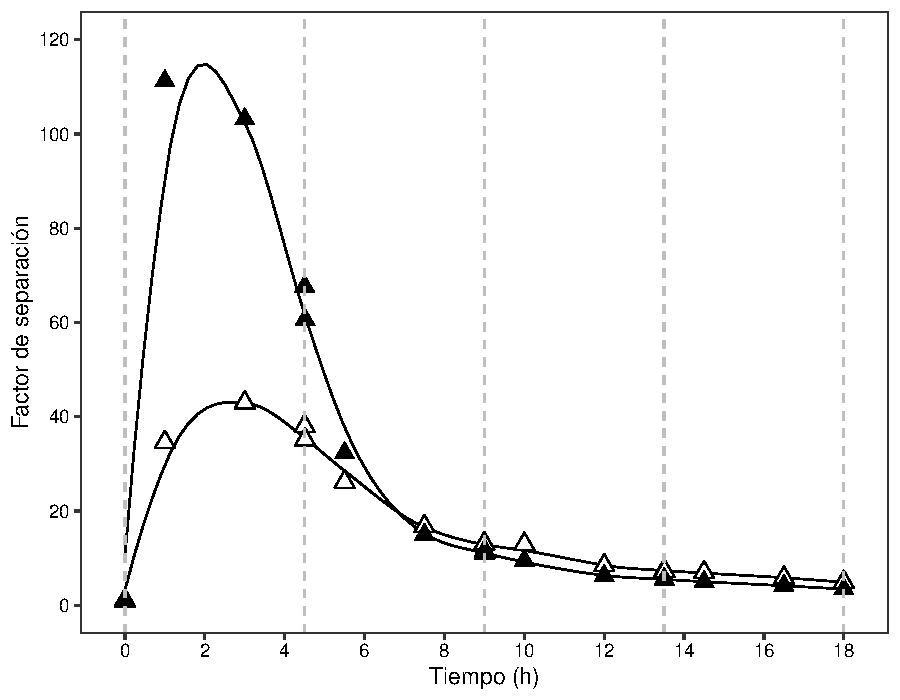
\includegraphics[width=0.6\textwidth, trim = {0cm 0cm 0 0}, clip]{chap5/figures/SW_Sep.pdf}
    \caption[Factor de separación de ion litio frente a sodio y potasio usando agua de mar natural.]{Factores de separación en función del tiempo para la concentración de ion litio usando agua de mar natural: (\protect\triangleupblck) \ce{Li+}/\ce{K+} y (\protect\triangleupwht) \ce{Li+}/\ce{Na+}. Las líneas descontinuas verticales corresponden al inicio o al final de cada ciclo.}
    \label{fig:SWselec}
\end{figure}

El factor de concentración de ion litio en agua de mar es 1.73 luego de cuatro ciclos de extracción. La eficiencia general de este proceso es de al rededor del 43\%, significativamente menor a la reportada en la Sección \ref{sec:idealconc} (64\%).


%\subsection{Resumen}


\clearpage\ChapBib{chap5/results}